	\documentclass[10pt,oneside]{CBFT_book}
	% Algunos paquetes
	\usepackage{amssymb}
	\usepackage{amsmath}
	\usepackage{graphicx}
% 	\usepackage{libertine}
% 	\usepackage[bold-style=TeX]{unicode-math}
	\usepackage{lipsum}

	\usepackage{natbib}
	\setcitestyle{square}

	\usepackage{polyglossia}
	\setdefaultlanguage{spanish}
	



	\usepackage{CBFT.estilo} % Cargo la hoja de estilo

	% Tipografías
	% \setromanfont[Mapping=tex-text]{Linux Libertine O}
	% \setsansfont[Mapping=tex-text]{DejaVu Sans}
	% \setmonofont[Mapping=tex-text]{DejaVu Sans Mono}

	%===================================================================
	%	DOCUMENTO PROPIAMENTE DICHO
	%===================================================================

\begin{document}

% =================================================================================================
\chapter{Conjuntos estadísticos}
% =================================================================================================


\section{Mecánica estadística. Boltzmann y teoría cinética}

Estaremos pensando en un hamiltoniano para muchas partículas (dinámica real)
\[
	H = \sum_i \frac{p^2}{2m} + \sum_{i < j} v_{ij}(|v_i-v_j|) + \sum_i U_i
\]

Sistema diluido. Las colisiones a un tiempo fijo son entre dos partículas; no entre más.
También lo garantiza esto la forma del potencial que se esfuma rápidamente a gran distancia.
Los procesos colisionales se definirán en base a $\sigma$, la sección eficaz, que no es otra cosa
que una probabilidad de transición.

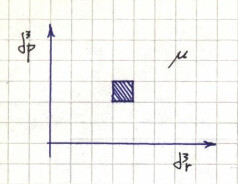
\includegraphics[scale=0.5]{images/1606329227.jpg}

Con normalización
\[
	N = \int \int f(r,p,t) d^3r d^3p
\]
donde se integra en el espacio de fases.
El gas ideal es la aproximación más baja; el $\sigma = 0$ porque no colisiona.
Consideremos un flujo libre
\[
	(r,p) \to ( r + v \delta t, p + F \delta t )
\]
En ausencia de colisiones, $f$ se consderva. Pero si hay colisiones tiene que variar

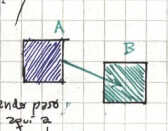
\includegraphics[scale=0.5]{images/1606329231.jpg}
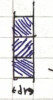
\includegraphics[scale=0.5]{images/1606329234.jpg}


En cada celda pueden convivir diferencias de momentos muy grnades entre partículas.
En el primer pic cuando paso dde aquí a aquçi si alguna partícula chocca, se modifica el $p$ de modo
que no llega a B. Posiciones cercanas y momentos (?) diferentes darán colisiones. 
En el segundo pic, estas colisionan: mismo espacio de configuración pero momento desigual

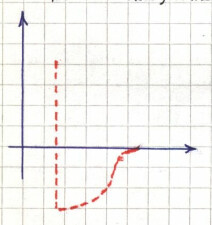
\includegraphics[scale=0.5]{images/1606329237.jpg}
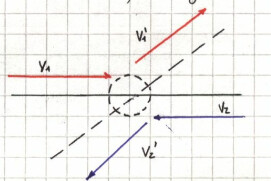
\includegraphics[scale=0.5]{images/1606329239.jpg}

Tenemos colisiones directas (asociadas a las que despueblan la celda) y colisiones inversas (asociadas
a las que pueblan la celda). La pérdida o ganancia se refiere a un salto en $\vb{p}$.
Finalmente, se tiene la ecuación de Boltzmann
\[
	\dpare{f}{t}{\text{coll}} = \int \int ( f' f'_1 - f f_1) V \sigma(V) d^2v_1 d\Omega.
\]

{\bf suelto}

El equilibrio corresponde a 
\[
	f_0(p_1) f_1(p_2) = f_0(p_1') f_1(p_2')
\]
que proviene de pedir $df/dt = 0$.
Considero, antes y después de la colisión, que estoy fuera del rango de interacción.
La distribución de Maxwell-Boltzmann (solución de equilibrio de la ecuación de Boltzmann).

\subsection{Teoría cinética}

La ecuación de transporte de Boltzmann
\[
	\left( \dpar{}{t} + \frac{\vbp}{m} \nabla_x + \vb{F}\Nabla_p \right) f(\vbx,\vbp,t) =
	\dpare{f}{t}{\text{coll}} 
\]
que vale para una situación estacionaria, donde no hay fuerzas externas $f(\vbx,\vbp,t) \to f(\vbp) $ 
(que satisface el miembro derecho nulo de la anterior) y es homogéneo (¿?).
Esta es la ecuación para la función de distribución.
Esto conduce a
\[
	f_0(\vbp) = \frac{ n }{( 2 \pi m k T )^{3/2}} \euler^{- (\vbp - \vbp_0)^2 / (2mkT)},
\]
que es la distribución de Maxwell-Boltzmann y en función de la velocidad,
\[
	f_0(\vbv) = n \Frac{ m }{2 \pi k T }^{3/2} \euler^{- m (\vbv - \vbv_0)^2 / (2kT)},
\]

Pero los ejercicios en general tienden campos externos. Los resuelvo con una perturbación
\[
	f = f_0 + f_1
\]
donde $f_0$ es MB y la otra es algo. Se requiere entonces la función de distribución de la perturbación,
que se hará considerando que $f_1 \ll f_0$
\[
	\left( \dpar{}{t} + \frac{\vbp}{m} \nabla_x + \vb{F}\Nabla_p \right) (f_0+f_1) =
	\dpare{f}{t}{\text{coll}} \approx -\frac{f_1}{\tau}
\]
donde $\tau$ es un tiempo característico medio entre colisiones.
Además se usará la hipótesis de equilibrio local la aforma de la distribución es siempre la de Boltzmann
en todo punto pero cambiand de punto a apunto $n, T, \vm{\vbv}$ que son funciones de $\vbx$ y, eventualmente,
del tiempo.

Sin embargo, pensaremos que estas variaciones serán suaves y relacionadas en el tiempo con el $\tau$.
Las variaciones de $f_1$ serán muy pequeñas. A igual orden, podemos pensar que
\[
	\left( \dpar{}{t} + \frac{\vbp}{m} \nabla_x + \vb{F}\Nabla_p \right) f_0 \approx -\frac{f_1}{\tau}
\]
con 
\[
	\dpare{f}{t}{\text{coll}}  = 0
\]

\begin{ejemplo}{\bf Problema 5}

Tenemos la situación ilustrada en la figura debajo

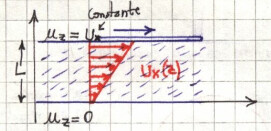
\includegraphics[scale=0.5]{images/1606329328.jpg}

donde se tiene
\[
	u_x(z) = \frac{u_x}{L} z
\]
con $\vm{v_x} = u_x(z)$.

A un plano dado la parte inferior retrasa a la parte de arriba. Para mantener el perfil hay que meter
energía que se va en el rozamiento.
La fuerza experimental por el fluido superior en la unidad de tiempo
\[
	f_\text{fricción} = - \mu \dpar{u_x}{z}
\]
donde $\mu$ es la constante de viscosidad.

Hay intercambio de partículas es a ritmo constante por el supuesto flujo laminar

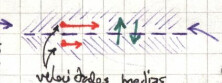
\includegraphics[scale=0.5]{images/1606329331.jpg}

lo que no está balanceado es el flujo de momentos; eso es lo que genera el frenado.
La cantidad transportada es $ m (v_x - u_x)$ donde la primera es la velocidad de las partículas, y
el flujo efectivo será $n (v_z - u_z )$
\[
	f_\text{fricción} = m n ( v_x - u_x ) (v_z - u_z )
\]
donde $u_x, u_z$ son velocidades medias. Entonces
\[
	P_{zx} = m n \vm{ (v_x - u_x) v_z }
\]
donde $\vm{u_z}=0$ pues no hay flujo neto en la dirección $\hat{z}$. Es el flujo en $\hat{z}$ de vector
$\vbp$ en $\hat{x}$.

\[
	f = f_0 ( v_x - u_x(z), v_y,m v_z ) + f_1
\]
y pensando en el estacionario y sin fuerzas externas
\[
	\frac{\vbp}{m} \nabla_x f = \dpare{f}{t}{\text{coll}}
\]
\[
	v_z \dpar{f_0}{z} = - \frac{f_1}{\tau} = - v_z \dpar{f_0}{U_x}(U_x,U_y,U_z) \dpar{U_x}{z}
\]
con $U_x = v_x - u_x(z)$ y $u_j=v_j$ para $j=y,z$.
De manera que ahora es
\[
	f = f_0 + \tau v_z \dpar{f_0}{U_x} \dpar{U_x}{z}
\]
y debo estimar
\[
	P_{zx} = m n \vm{U_zU_z}_{f_0+f_1}
\]
pero $\vm{U_xU_z}_{f_0} = 0$ por la simetría de la distribución de MB.
\[
	P_{zx} = n m \tau \int d^3 U \: U^2_z U_x \dpar{f_0}{U_x} \dpar{U_x}{z} =
	- n \tau m^2 \beta \dpar{U_x}{z} \vm{ U_z^2 U^2_x}_{f_0}
\]
\[
	\vm{ v_z^2 }_{f_0} = \frac{ k T }{m} = \frac{1}{\beta m} \qquad 
	P_{zx} = - n \tau m^2 \beta \dpar{U_x}{z} \frac{1}{\beta^2 m^2 }
\]
\[
	P_{zx} = - \frac{n \tau}{\beta} \dpar{U_x}{z}
\]
donde el factor que está pegado a la derivada es la viscosidad $\eta$ de manera que
\[
	\eta = n \tau k T.
\]

La otra parte pide calcular una conductividad

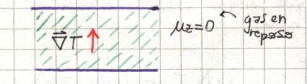
\includegraphics[scale=0.5]{images/1606329338.jpg}

y quiero ver el flujo de calor (flujo de energía cinética)
\[
	\bar{Q} = n \frac{m}{2} \vm{ \vbv v^2 }
\]
forzamos la existencia de un gradiente de temperatura y llegamos a la misma ecuación
\[
	\left( \dpar{}{t} + \frac{\vbp}{m} \nabla_x + \vb{F}\Nabla_p \right) f_0 = - \frac{f_1}{\tau}
\]
y con 
\[
	f_1 = - \tau v_x \dpar{f_0}{z}
\]
es
\[
	f_0 = n(z)\Frac{ m \beta(z) }{ 2 \pi }^{3/2} \euler^{ - \beta(z)/2 m ( \vbv - \vm{\vbv})^2}
\]
donde la velocidad media es nula por estar en reposo.

Usando regla de la cadena,
\[
	f_1 = - \frac{\tau}{n} \dtot{n}{z} f_0 v_z - \tau v_z \dpar{f_0}{\beta} \dpar{\beta}{z}
\]
y queremos ver si las derivadas $\partial n/\partial z$ y $\partial \beta / \partial z$ están relacionadas.
Como estoy en equilibrio y no hay movimiento neto,
\[
	\vm{v_z}_{f_0+f_1} = 0 \quad \to \quad \vm{v_z}_{f_1} = 0
\]
y $\int f_1 v_z d^3v = 0$ donde se puede amasar para llegar a
\[
	\dtot{n}{z} = - k \beta h \dtot{T}{z},
\]
luego
\[
	f_1 = \frac{\tau}{T} \dtot{T}{z} \left[ f_0 + \frac{1}{kT}\dpar{f_0}{\beta} \right] v_z
\] 
y
\[
	Q_z = \frac{1}{2} n m ( \vm{ v^2_x v_z } + \vm{ v^2_y v_z } + \vm{ v_z^3 } )
\]
\[
	Q_z = \frac{\tau}{T} \dtot{T}{z} \frac{ n m }{2} \left( 1 + \frac{1}{kT}\dpar{}{\beta} \right)
	\int d^3v ( v_x^2 v_z^2 + v_y^2 v_z^2 + v_z^4 ) f_0
\]
donde la integral debería dar $ 5 /m^2 (kT)^2$, entonces
\[
	Q_z = - \frac{5}{2}  \tau n k^2 T  \dtot{T}{z} \equiv \kappa \dtot{T}{z}
\]
y podemos considerar el cociente
\[
	\frac{\kappa}{\eta} = \frac{ 5/2 \tau n T k^2 }{ n \tau \kappa T } = \frac{5}{2}k
\]

La aproximación consiste en poner $f=f_0 +f_1$ y 
\[
	\dpare{f}{t}{\text{col}} \sim - \frac{f_1}{\tau}
\]
que es la aproximación de tiempo de relajación.
 
\end{ejemplo}

\begin{ejemplo}{\bf Problema 6}

Estimar densidad de corriente. Los electrones no sienten el campo de los iones.
Planteamos la ecuación 
\[
	\dpar{f}{t} + \vbv \nabla_x f_0 + \frac{\vb{F}}{m}\nabla_p f_0 = -\frac{f_1}{\tau}
\]
con $\vb{E}=E\zver$ y $\vb{F}=-eE\zver$ de manera que $f_1 = - e E 2 \beta v_z f_0$
y el flujo que interesará calcular será $J_z = - n e \vm{ v_z } $.

\notamargen{Puede ser que no haga falta ir a $\tau$ si puedo tener algo que rompe 
la simetría de traslación; entonces meto $f_0(\vbx,\vbp)$.}

\end{ejemplo}





\subsection{Ensamble gibbsiano}

Dada una condición macroscópica ($U,V,N$) puedo construirme todos los estados compatibles con esa condición.
Tendré una densidad de estos estados en $\Gamma$.
Paredes reflectantes al 100\% implican conservación de la energía

Desde $\Gamma \to \mu$ (espacio de celdas discreto; un grano grueso)
\[
	\sum_i n_i = N
\]
de manera que un punto en $\Gamma$ va a una $f$ en $\mu$, y $f$ en $\mu$ va a un volumen en $\Gamma$
(muchos puntos en $\Gamma$). De manera que la $f$ con mayor volumen será la más probable.


Considero partículas distinguibles, y así se llega a
\[
	f_i \propto C \euler^{ - \beta \varepsilon_i }
\]

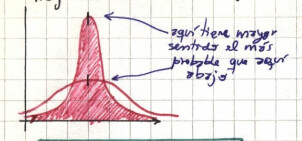
\includegraphics[scale=0.5]{images/1606329273.jpg}

\notamargen{Lo que cuenta es el ancho de la campana (figura).}


Queremos encontrar el extremo de $\Omega(n)$. Con $N\to\infty$ en Boltzmann la distribución MB es la dominante
(independientemente del hamiltoniano). La $\sigma$ es nula.

\section{Teorema H}

Si $H$ es constante en el tiempo entonces $f$ será constante. Se considera $H \equiv \int d^3v f \log (f)$
\[
	\dtot{H}{t} \leq 0,
\]
y esto define una flecha del tiempo.
Entonces como $H$ es siempre no positiva, $H$ será acotada y entonces se llega al mínimo y se queda ahí.
Pero esto es incompatible con el teorema de Poincaré, por ejemplo. Luego se vio que en realidad $H$ fluctúa.

Las ecuaciones de la mecánica (sistemas aislados no disipativos) son invertibles temporalmente.
El teorema H de Boltzmann parece ser violado si miramos en una escala de tiempo que no nos muestra
la \textit{picture} completa.

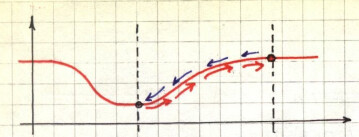
\includegraphics[scale=0.5]{images/1606329246.jpg}

Por el camino azul parece violar el tema de minimizar $H$ en el avance temporal.

\section{Ensamble}

Un ensamble es un conjunto de puntos en el espacio $\Gamma$.
Consideramos una condición de un sistema con $U,V,N$ entonces tendrá ciertos valores de $p,q$ (que
evolucionan en el tiempo como el hamiltoniano predice). Dará una cierta $\rho(p,t)$.
Tenemos el teorema de Liouville
\[
	\dpar{\rho}{t} + \sum_i \left[ \dpar{\rho}{p_i} \dot{p}_i + 
	\dpar{\rho}{q_i} \dot{q}_i \right] = 0
\]
y entonces la condición
\[
	\dtot{\rho}{t} = 0,
\]
nos habla de un {\it fluido} incompresible.
Entonces, la densidad de puntos en el espacio $\Gamma$ no varía. Los volúmenes se conservan; es una
consecuencia de los volúmenes aislados. No se crean ni aniquilan puntos.

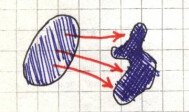
\includegraphics[scale=0.5]{images/1606329250.jpg}

Según ilustra la picture se conserva el número de puntos en la transformación.

La jerarquía BBGKY son unas ecuaciones acopladas que dan la evolución de las funciones de distribución
en función de las otras.

El ensmable microcanónico corresponde a $U,V,N$ fijos con paredes perfectamente reflectantes.
La condición sobre $U$ es que hay un mapeo de $\Gamma$ a $\mu$ que define un número de ocupación,
pero en esa transformación se pierde información microscópica; se pierde datos porque de un punto en
$\Gamma$ paso a unas celdas en $ \mu $.

Quiero exrtremar el número de ocupación y, con aproximación de Stirling mediante, se llega a
\[
	\tilde{f} = C \euler^{-\beta \epsilon},
\]
una distribución normal para la distribución más probable. Una distribución \textit{chancha} no nos da mucha
información mientras que una \textit{picuda}, en cambio, sí.

La cantidad
\[
	\rho(\{ \vec{q}_i, \vec{p}_i\},t) d^{3N}qd^{3N}p
\]
es el número de microestados en el elemento $d^{3N}qd^{3N}p$ al tiempo $t$ centrado en $q,p$.
Si los microestados son equiprobables $\rho \equiv cte.$. El conjunto $\{ \vec{q}_i, \vec{p}_i\}$ son
$6N$ coordenadas.
\[
	\Omega = \int p d^{3N}qd^{3N}p
\]
\notamargen{La integral $\Omega$ es imposible porque es difícil determinar el volumen de integración.}

XXX Dibujos XXXX

el volumen en  $\mathbb{\Gamma}$ es proporcional al número de microestados compatibles con $E,N$,
el volumen $ \mathbb{\Gamma}$ del macroestado es $\Omega\{ n_i \}$

$n_i = f_i d^3q d^3p$ es el número de partículas en una celda $i$ (con su $\vec{p}$ en $\vec{p} + d\vec{p}$
y con su $\vec{q}$ en $\vec{q} + d\vec{q}$ )

Un microestados determina una distribución $f$ que da un conjunto $\{ n_i \}$. Pero una $f$ determina muchos
microestados porque la función de distribución no distingue entre partículas (importan los números de 
ocupación); entonces una $f$ determina un volumen en $\mathbb{\Gamma}$.
\notamargen{Cada microestado tiene su $f$.}

Suponemos que todos los microestados en $\mathbb{\Gamma}$ son igualmente probables.
La $f$ que determina el mayor volumen en  $\mathbb{\Gamma}$ es la más probable. Suponemos que en el 
equilibrio el sistema toma la $f$ más probable.
Si $f_i$ es el valor de $f$ en cada celda $i$
\[
	f_i = \frac{n_i}{d^3p d^3q} \quad \text{promediada en el ensamble} \quad \bar{f}_i =  \frac{<n_i>}{d^3p d^3q}
	\quad \text{en el equilibrio}
\]
\notamargen{$f_i$ es la distribución para un miembro en el ensamble.}

Esta $\bar{f}_i$ es la de equilibrio, pero la cuenta no es fácil. Asumiremos que la $f$ de equilibrio es la más
probable (la de mayor volumen en  $\mathbb{\Gamma}$); entonces maximizaremos dicho volumen para hallarla.

Un microestado determina una $f$; diferentes microestados pueden determinar otras $f$ pero muchos coincidirán en
una misma $f$.

La $f$ en el equilibrio es la que tiene mayor cantidad de microestados (la más probable) pero 
\[
	\bar{f}_i =  \frac{<n_i>}{d^3p d^3q}
\]
es el promedio en el ensamble y no será exactamente igual a la $f_i$ del mayor volumen, salvo que el volumen de $f$
sea mucho mayor al ocupado por $f',f''$, etc.

Dado el volumen $\Omega \{ n_i\}$ extremaremos el mismo sujeto a las condiciones
\[
	E = \sum_i^K n_i e_i \qquad \qquad N = \sum_i^K n_i
\]
y llegamos a la $f$ de equilibrio que es $f_{MB}$.
\notamargen{Necesito $\Omega = \Omega \{ n_i\}$ para obtener el $\{ \tilde{n}_i\}$.}

El volumen $\Omega$ se escribe en función de los números de ocupación
\[
	\Omega \left( \{ n_i \} \right) = 
	\frac{N!}{\prod_i^K n_i!} \prod_i^K g_i^{n_i} \qquad 
	(i=1,2,...,K \quad \text{identifica celdas en}\;\mu )
\]
\[
	\Omega \left( \{ n_i \} \right) = N! \prod_i^K \frac{g_i^{n_i}}{n_i!}
\]
donde $g_i$ son los subniveles en que podríamos dividir la celda $K$; es por matemática conveniencia y para abarcar 
más casos (luego será $g_i=1 \forall i$).

El conjunto $\{ \tilde{n}_i\}$ que extrema $\Omega \left( \{ n_i \} \right)$ es el más probable y consideraremos
\[
	\{ \tilde{n}_i\} = < n_i >
\]
Estaremos pensando que cuando $N \to \infty$ la mayor parte de los microestados van a una distribución $f_{MB}$

{\bf Conceptos}

La idea  es que tendremos $N$ encerradas en $V$ con $N \sim 10^23$ y será $N \to \infty$ y $V \to \infty$ (esto
es el llamado límite termodinámico).
Con estos límites extensivos (son proporcionales al tamaño) o intensivos (son independientes de $N,V$ )

Un macroestado es del punto de vista termodinámico. Especificamos unas pocas variables ($N,V,E,T$)
Un microestado es una especificación de seis grados de libertad $(3 N_q, 3 N_p)$ y claramente un macroestado
es compatible con muchos microestados.

Un ensamble, en la visión de Gibbs, es el conjunto de microestados compatibles con un dado macro estado.

\begin{itemize}
 \item Microcanónico: usado para analizar sistemas aislados. Con $E,V,N$ fijos.
 \item Canónico: usado para analizar sistemas en equilibrio con un baño térmico. Con $V,N,T$ fijos.
 \item Gran canónico: usado para analizar sistemas que además intercambian partículas. Con $\mu,V,T$ fijos.
\end{itemize}

En el límite termodinámico los tres ensambles son equivalentes.

La cantidad de micro estados compatibles con el macroestado NVE fijo se denota
\[
	\text{\#} \mu\text{-estados con un M-estado } \equiv \Gamma(N,V,E)
\]

Confiamos en un postulado de equiprobabilidad a priori: todos los microestados son igualmente probables
(microscópicamente hablando)

\subsection{Visión [de statistical mechanics - Pathria]}

Sean dos sistemas en equilibrio. Llegan al equilibrio en algún momento


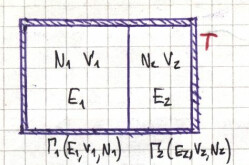
\includegraphics[scale=0.5]{images/1606329365.jpg}

La energía total $ E_T = E_1 + E_2 $ es una constante y el número de estados
\[
	\Gamma(E) =  \Gamma_1(E_1) \Gamma_2(E_2) = \Gamma_1(E_1) \Gamma_2(E_T-E_1).
\]
En el equilibrio, ¿Cuánto valen $E_1$ y $E_2$? Para esto se asume un postulado:

El equilibrio se da cuando el sistema llega al macroestado más probable. Este macroestado será el que
tenga mayor cantidad de microestados.

Entonces, el sistema llegará a $E_1,E_2$ tales que $\Gamma_2(E_T-E_1)$ sea máxima. Buscamos esa
condición de maximización,
\[
	\dpare{\Gamma_1(E_1)}{E_1}{E_1=\bar{E}_1} \Gamma_2(E_1) = 
	\Gamma_1(E_1) \dpare{\Gamma_2(E_2)}{E_2}{E_2=\bar{E}_2} 
\]
\[
	\dpar{\log \Gamma_1(E_1)}{E_1} = \dpar{\log \Gamma_2(E_2)}{E_2}
\]
y definiendo 
\[
	\beta = \dpare{\log \Gamma(E,N,V)}{E}{E=\bar{E}} 
\]
se tiene que la condición de equilibrio es
\[
	\beta_1 = \beta_2.
\]

Pero en termodinámica el equilibrio era con $T_1=T_2$ donde 
\[
	\frac{1}{T} \equiv \dpare{S}{E}{N,V},
\]
de manera que podemos plantear la siguiente equivlaencia
\be
	S = k \log \Gamma(E,N,V),
	\label{boltzmann_relation}
\ee
que es la relación de Boltzmann.

Esto vincula la mecánica estadística con la termodinámica. Nos lleva a la tercera ley de la termodinámica.
Entonces si $S = 0$ se tiene $\Gamma=1$ un único estado microscópico. En caso contrario, si $S$ es
grande tenemos un sistema más desordenado, $\Gamma$ grande, tendrá muchos estados microscópicos
asociados.

En el formalismo del microcanónico nos interesará en principio la función de partición microcanónica
$Z_{\mu C} = \Gamma (E,N,V)$ dado el vínculo en \eqref{boltzmann_relation} se tienen
\[
	\dpare{S}{E}{N,V} = \frac{1}{T} \qquad \qquad \dpare{S}{V}{E,V} = \frac{P}{T}
\]

Lo que sería bueno es saber cómo calcular $\Gamma$
\[
	\Gamma(E) = \sum_{\mu-\text{estados}} 1 \qquad P_{\mu(E)} = \frac{1}{\Gamma(E)}
\]
donde el ``1'' es la densidad unitaria por la equiprobabilidad.
En el continuo, un microestado es un punto en el espacio $6N$ dimensional $\Gamma$.
Así pensado, debo tener en cuenta una función densidad en $\mathbb{\Gamma}$ donde:
\[
	f(p,q) d^{3N}q d^{3N}p
\]
es el número de puntos del ensamble contenidos en un elemento de volumen $d\Gamma = d^{3N}q d^{3N}p $.

Parece lógico suponer que si tenemos un observable macroscópico vlaga que 
\[
	\vm{\text{obs}} =
	\frac{\int f( p, q) \; \text{obs} \; d^{3N}p d^{3N}q}{\int f(p,q) d^{3N}p d^{3N}q } 
\]
el observable visto en la macroscopía es un valor medio.

Para un microcanónico
\[
	f(p,q) = \begin{cases}
			\text{constante} \quad &\text{El } H \text{ verifica }   E+\Delta > H > E \\
			0                \quad &\text{En otro caso}
	         \end{cases}
\]
donde $\Delta \lll E$. Luego, se tiene
\[
	\Gamma(E) = \frac{\text{Volumen del ensamble en $\mathbb{ \Gamma}$}}{\text{Volumen que ocupa el microestado}}
\]
y
\[
	\Gamma(E) = \frac{1}{h^{3N}} \int_{E < H < E+\Delta} \kern-2em 1 \; d^{3N}p d^{3N}q \qquad 
	\Sigma(E) = \frac{1}{h^{3N}} \int_{H < E } \kern-0.5em 1 \; d^{3N}p d^{3N}q
\]
donde $h^{3N}$ es la constante de Planck de adimensionalización y representando un volumen mínimo
dada la incertidumbre. Las dos cantidades mostradas difieren en un término que va como $\log(N)$ y
que muere en el límite termodinámico
\[
	\frac{\log(N)}{N} \to 0 \qquad \text{ si } \qquad  N \to \infty
\]

Es más cómodo calcular $\Sigma(E)$ que $\Gamma(E)$.
\[
	\Gamma(E) = \Sigma(E+\Delta) - \Sigma(E)
\]

% =================================================================================================
\section{Microcanónico}
% =================================================================================================

\subsection{Solución de equilibrio}

La solución de equilibrio satisfacía
\[
	f(p_1) f(p_2) = f(p_1') f(p_2')
\]
\[
	\log f(p_1) + \log f(p_2) = \log f(p_1') + \log f(p_2')
\]
que luce como una ley de conservación y admite como solución
\[
	\log f(p) = A m + \vb{B}\cdot \vb{p} + C|\vb{p}|^2 
	\qquad (A,\vb{B},C \text{ctes. adimensionales})
\]
que lista los {\it invariantes colisionales}. Completando cuadrados
\[
	f \propto C_1 \euler^{-C_2(\vb{p} - \vb{p}_0)^2}
\]

La expresión completa se ajusta con 
\[
	n = \int f(\vb{p},t) d^3p
\]
donde el $\vb{p}$ de una partícula es
\[
	<\vb{p}> = \frac{\int f(\vb{p}) \vb{p} \; d^3p d^3q}{\int f(\vb{p}) \; d^3p d^3q } = 
	\frac{1}{n} \int f(\vb{p}) \; \vb{p} \; d^3p
\]
\notamargen{El cociente es $\vb{P}/N$.}
y la energía por partícula
\[
	<e> = \vm{e} = \frac{\int f(\vb{p}) \; \vb{p}^2/ (2m) \; d^3p d^3q}{\int f(\vb{p}) d^3p d^3q } = 
	\frac{1}{n} \int f(\vb{p}) \frac{ \vb{p}^2 }{ 2m } \; d^3p
\]

Finalmente se llega a 
\[
	f(\vb{p}) = \frac{n}{(2\pi m k T)^{3/2}} \euler^{- \frac{( \vb{p} - \vb{p}_0 )^2}{2mkT} }
\]

que es la función de distribución de momentos de Maxwell-Boltzmann.
\notamargen{Solución de equilibrio de la ecuación de transporte}

\[
	\text{(presión ideal)} \qquad p = \frac{2}{3} \frac{U}{V} = \frac{2}{3} n \epsilon =
	\frac{2}{3} n \frac{3}{2} k T = nkT 
\]

\subsection{Método de la distribución más probable}

Con este método también llegamos a $f_{MB}$ pero extremandolo el volumen $\Omega(\{ n_i \})$ que ocupa en el espacio
$\mathbb{\Gamma}$ sujeto a los vínculos $E = \sum_i n_i e_i$ y $N = \sum_i n_i $.

Luego podemos estimar qué tan probable es la distribución de MB (la más probable) considerando
(ASUMIMOS)
\[
	\text{los \# de ocupación de MB} \quad \tilde{n}_i \cong <n_i> \quad \text{el promedio en el ensamble}
\]
pero esto sólo valdrá si las desviaciones son pequeñas; es decir si $f_{MB}$ es muy muy probable.

Calculamos la desviación cuadrática (varianza) se tiene 
\[
	<n_i^2> - <n_i>^2 = g_i \dpar{<n_i>}{g_i}
\]
donde se usó que 
\[
	<n_i> = \frac{\sum_{\{ n_j\}} n_i \Omega\{ n_j\} }{\sum_{\{ n_j\}} \Omega\{ n_j\}}
\]

Suponiendo que $ <n_i> \approx \tilde{n}_i$ entonces $ <n_i>  \propto f_{MB}$ con lo cual se tiene también 
\[
	<n_i^2> - <n_i>^2 \cong \tilde{n}_i
\]
\notamargen{como $ g_i \dpar{\tilde{n}_i}{g_i} = \tilde{n}_i $}
y las fluctuaciones relativas
\[
	\sqrt{<\left( \frac{m_i}{N}\right)^2 > - <\left( \frac{m_i}{N}\right) >^2 } \cong 
	\sqrt{ \frac{ \tilde{n}_i/N }{N} }\to_{N\to\infty} 0
\]

En el límite termodinámico MB es totalmente dominante.

\subsection{Hipótesis ergódica}

La trayectoria individual de casi cualquier punto en el $\Omega$ pasa, con el tiempo, a través de todos los
puntos permitidos del espacio $\mathbb{\Gamma}$. Si esperamos lo suficiente, todos los microestados posibles
son visitados.

Considerando un $H$ independiente del tiempo. Coinciden los promedios:
\begin{itemize}
 \item Seguir cada trayectoria, resolviendo las ecuaciones de movimiento hasta tiempo infinito.
 \item Calcular valor medio en el espacio $\Gamma$
\end{itemize}


\subsection{Observaciones sobre el microcanónico}

\[
	\Gamma(E) = \int_{E < \Ham < E + \Delta E} \rho d^{3n}p d^{3n}q \qquad 
	\Sigma(E) = \int_{\Ham < E} \rho d^{3n}p d^{3n}q
\]
entonces 
\[
	\Gamma(E) = \Sigma( E + \Delta E ) - \Sigma( E ) \cong \dpar{\Sigma( E )}{E}\Delta E  
	\qquad \text{si}\; \Delta E \ll E
\]
$\Delta E$ es el {\it paso} entre medidas de energía 
\[
	\Gamma(E) = \Gamma_1(E_1) \Gamma_2(E_2) \qquad \text{(1 y 2 son subsistemas)}
\]
\[
	E = E_1 + E_2 \Rightarrow \Gamma(E) = \sum_i^{E/\Delta E} \Gamma_1(E_i)\Gamma_2(E-E_i)
\]
siendo $E/\Delta E$ el número de términos tales que se cumple $ E = E_1 + E_2 $.
Si se da $ N_1 \to \infty $ y $ N_2 \to \infty $ será
\[
	\log \Gamma_1 \propto N_1 \quad \log \Gamma_2 \propto N_2 \quad E \propto N_1 + N_2
\]
luego $\log(E/\Delta E)$ es despreciable pues $\Delta E$ es constante y entonces
\notamargen{$\log(E/\Delta E) \propto \log(N)$ pues $E\propto N$ y $\Delta E$ cte.}
\[
	S(E,V) = S(\tilde{E}_1,V_1) + S(\tilde{E}_2,V_2) + \mathcal{O}(\log[N])
\]
con lo cual la mayoría de los microestados tienen los valores $\tilde{E}_1$ y $\tilde{E}_2$ de energía.

Asimismo
\[
	\delta( \Gamma_1(\bar{E}_1)  \Gamma_2(\bar{E}_2) ) = 0 \qquad \delta( \bar{E}_1 + \bar{E}_2 ) = 0
\]
\[
	\delta\Gamma_1 \Gamma_2 + \Gamma_1 \delta \Gamma_2 = 0 \quad \delta( \bar{E}_1 ) = -\delta ( \bar{E}_2 )
\]
\[
	\frac{\delta\Gamma_1}{\bar{E}_1}\Gamma_2 = \Gamma_1\frac{\delta\Gamma_2}{\bar{E}_2} \Rightarrow 
	\frac{1}{\Gamma_1} \dpar{\Gamma_1}{\bar{E}_1} = \frac{1}{\Gamma_2} \dpar{\Gamma_2}{\bar{E}_2} 
\]
\[
	\dpar{}{\bar{E}_1}\left( k\log \Gamma_1(\bar{E}_1) \right) = 
	\dpar{}{\bar{E}_2}\left( k\log \Gamma_1(\bar{E}_2) \right)
\]
\[
	\left. \dpar{}{{E}_1}S(E_1)\right|_{\bar{E}_1} = \left. \dpar{}{{E}_2}S(E_2)\right|_{\bar{E}_2}
	\equiv \frac{1}{T} \qquad \text{en equilibrio} \; T_1 = T_2
\]

La $T$ es el parámetro que gobierna el equilibrio entre partes del sistema.

La idea es que dado un sistema de $E = E_1 + E_2$, sistema compuesto de dos subsistemas, hay muchos valores
1,2 tales que $E = E_1 + E_2$ pero hay una combinación que maximiza $\Gamma(E)$ y es
\[
	\Gamma_{Max}(E) = \Gamma_1(\bar{E}_1)  \Gamma_2(\bar{E}_2) 
\]
\notamargen{El sistema es $E,N,V$ y yo lo pienso compuesto de dos partes $E_1,N_1,V_1$ y $E_2,N_2,V_2$.}

Luego, con $N_1, N_2 \to \infty$ se da que la mayoría de los sistemas tendrán $E_1=\bar{E}_1$ y $E_2=\bar{E}_2$.
Esa configuración, por supuesto, maximiza la entropía $S=k\log(\Gamma)$.

El hecho de que $\Delta S> 0$ para un sistema aislado lo vemos considerando que tal sistema sólo puede variar
$V$ (creciendo, como en la expansión libre de un gas), luego $V_F > V_I$ y entonces
\[
	\Sigma(E) = \int_{\Ham < E} \rho d^{3N}p d^{3N}q \underbrace{\longrightarrow}_{\text{Si aumento el volumen}}
	\Sigma(E)' = \int_{\Ham < E} \rho d^{3N}p d^{3N}q
\]
\notamargen{Será un número mayor porque el dominio de integración en $q$ es mayor.}
\[
	\Sigma(E)' > \Sigma(E) \qquad \Rightarrow \qquad \Delta S > 0
\]

Equipartición implica 
\[
	\left< x_i \dpar{\Ham}{x_j} \right> = \delta_{ij} k T
\]
y entonces
\[
	\left< p_i \dpar{\Ham}{p_i} \right> = \left< p_i \dot{q}_i \right> = kT 
\]
y
\[
	\left< q_i \dpar{\Ham}{q_i} \right> = \left< q_i \dot{p}_i \right> = kT 
\]
\[
	\left< \sum_i^{3N} q_i \dpar{\Ham}{q_i} \right> =  \sum_i^{3N} \left< q_i \dpar{\Ham}{q_i} \right> =
	\sum_i^{3N} k T = 3 N k T
\]
entonces llegamos al virial,
\[
	\sum_i^{3N} \left< q_i \dot{p}_i \right> = 3 N k T.
\]

Considerando un hamiltoniano armónico,
\[
	\left< \Ham \right> = E \qquad \text{con} \quad \Ham = \sum_i^{3N} a_i p_i^2 + b_i q_i^2
\]
\[
	p_k \dpar{\Ham}{p_k} = 2 a_k p_k^2 \qquad q_k \dpar{\Ham}{q_k} = 2 b_k q_k^2
\]
de modo que 
\[
	\Ham =  \sum_i^{3N} \frac{1}{2} p_k \dpar{\Ham}{p_k} + \frac{1}{2} q_k \dpar{\Ham}{q_k}
\]
\[
	\left< \Ham \right> =  \sum_i^{3N} \frac{1}{2} \left< p_k \dpar{\Ham}{p_k}\right> +
		\frac{1}{2} \left< q_k \dpar{\Ham}{q_k} \right>
\]
y si $f$ es el número de constantes $a_k,b_k$ no nulos
\[
	\left< \Ham \right> =  \frac{1}{2} f k T
\]

Si fuesen todas no nulas entonces
\[
	\left< \Ham \right>  = 3 N k T.
\]

{\bf Suelto para reprocesar}

Ensambles calcula valores medios sumando sobre todos los
\[
	N \to  \infty, \quad V \to \infty \qquad \frac V N = v
\]

Para un sistema aislado, equiprobabilidad a priori, $\rho=$ cte es solución si ajusta a $P,V,T$
\[
	S(U,V) = k \log T(U)
\]
donde supondremos que $U$ es aditiva. Como $E=E_1 + E_2$ el volumen en el espacio de fases
\[
	\Gamma(U) = \sum_{i j} \Gamma_1(E_1)\Gamma_2(E - E_1)
\]
de dos sistemas separados y luego reunidos.
En el equilibrio $T_1=T_2$

Además el crecimiento de la entropía en el sistema aislado. Expansión libre: $q$ crece entonces 
$\Gamma$ crece.

Pero por Liouville $V_\Gamma$ no varía de modo que la evolución en el espacio de fases hará que
ciertos estados sean inalcanzables ({\it mixing}).

Tenemos la paradoja de Gibbs porque hemos estado considerando partículas indistinguibles; entonces
al considerar la indistinguibilidad debemos sumar menos (es decir que hay que dividir por un
factor). Sin embargo, la indistinguibilidad es un concepto no clásico.
Es $ \Delta S > 0 $ con distinguibles y $ \Delta S = 0 $ si son distinguibles.
Esta corrección por distinguibilidad no tiene fundamento clásico.

Boltzmaniones: partículas en las cuales uso todas las herramientas clásicas y al final solo
corregimos con un factor $1/N!$ por indistinguibilidad.


\subsection{Fenómenos de transporte}

Un gas clásico verifica
\[
	\frac{\hbar}{\sqrt{2 m k T}} \Frac{N}{V}^{1/3} \sim 0.0004 \ll 1
\]
donde el primer factor es la longitud de onda de DeBroglie de modo que es un ratio 
del tipo $\lambda / \ell$ porque el segundo término es la inversa del volumen por
partícula elevado a la un tercio.

Entonces
\[
	f(\vb{x}, \vb{p}, t ) d^3x d^3p 
\]
es el número de partículas que se hallan entre $\vb{x}, \vb{x} + d \vb{x}$ y con 
$(\vb{p}, \vb{p} + d \vb{p} )$ en un tiempo $t$.

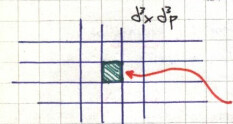
\includegraphics[scale=0.5]{images/1606329279.jpg}


Hay un número grande de partículas en cada celda. Es un diferencial no matemático (un {\it cachito})
puesto que no tenderá a cero.

\begin{ejemplo}{\bf Problema 3}

Se consider un gas clásico de $N$ partículas
\[
	\int \int f(\vb{x}, \vb{p}, t ) d^3x d^3p = N \qquad \qquad 
	\int f(\vb{x}, \vb{p},t) d^3p = n
\]
y asociamos a una partícula una $\alpha(\vb{x}, \vb{v}, t)$ donde ($\alpha$) serán cantidades extensivas.

El flujo de $\alpha$ se ilustra así
 
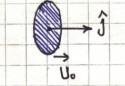
\includegraphics[scale=0.5]{images/1606329282.jpg}

de modo que
\[
	\vm{\alpha}(\vb{x},t) = \frac{\int \alpha(\vb{x},\vb{p}, t) f(\vb{x},\vb{p},t) d^3p}
	{\int f(\vb{x}, \vb{p},t) d^3p} =
	\frac{1}{n} \int \alpha(\vb{x},\vb{p}, t) f(\vb{x},\vb{p},t) d^3p
\]
Y entonces,
\[
	\hat{j} \cdot \int d^v \alpha(\vb{v}-\vb{u}_0) f(\vb{x},\vb{p},t) =
	\hat{j} \cdot \vm{ \vb{v}-\vb{u}_0 \cdot \alpha } n(\vbx,t),
\]
de manea que el flujo de $\alpha$ es todo lo que multiplica a la dirección $\hat{j}$.

Recordemos la consideración usual microscópica para el flujo ilustrada a continuación:

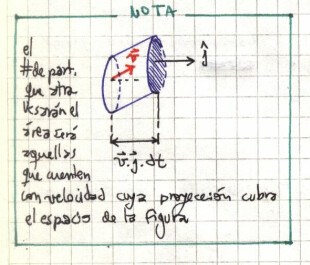
\includegraphics[scale=0.5]{images/1606329287.jpg}

{\bf Densidad de corriente}

Será la carga por unidad de tiempo en una superficie
\[
	\phi_e = n(\vb{x},t) \cdot \vm{\hat{j}\cdot \vb{v}_q}
\]
o bien 
\[
	\vec{\phi}_e =  n(\vb{x},t) \vm{\vb{v}_q}
\]
luego será $\phi_e = n q \vm{ \hat{j} \cdot \vb{v} }$

{\bf Flujo térmico (calor)}
\[
	Q = n(\vb{x},t) \vm{ 1/2 m v^2 \vb{v} }
\]
donde $ \alpha = 1/2 m v^2 $ es la densidad de energía cinética (asociada a temperatura)

{\bf $P_{ij}$ flujo de momento}

\[
	\alpha(\vbx, \vb{v}, t) = m ( \vm{v}_i - \vm{v_i} )
\]
\[
	P_{ij} = m \vm{  (\vm{v}_i - \vm{v_i}) v_j } n
\]
y se ve que el flujo de momento es claramente un tensor.

Sea la distribución $f(\vbx, \vbv, t )$ y entonces quiero llegar al equilibrio y ver que ya no
depende del tiempo. La ecuación que define la evolución temporal de $f$ es la ecuación de
Boltzmann.

Si no hay colisiones debe valer
\[
	\vbp_i \to \vbp_i + \vb{F} \delta t \qquad 
	\vbx_i \to \vbx_i + \vbv \delta t
\]
pero el número de partículas se mantiene constante
\[
	f(\vbx,\vbp, t) d^3x d^3p = f(\vbx',\vbp', t') d^3x' d^3p'
\]
y con sistema hamiltoniano es $ d^3x d^3p = d^3x' d^3p'$.
Lo que estamos diciendo es que por colisiones hay partículas que chocan y va a parar a otro $\delta V$
y hay otras que chocan y por ello vienen a parar a este $\delta V$; hay ganancia y pérdida.
Entonces,
\[
	f(\vbx,\vbp, t) = f(\vbx + \vbv \delta t,\vbp + \vb{F} \delta t, t + \delta t)
\]

Si $\delta t=0$ se tiene $df/dt=0$ de lo cual deducimos
\[
	\left( \dpar{}{t} + \frac{\vbp}{m} \nabla_x + \vb{F}\Nabla_p \right) f(\vbx,\vbp,t) = 
	\begin{cases}
	 0 \quad \text{ No hay colisiones}\\
	 \dpar{f}{t} \quad \text{ Hay colisiones}\\
	\end{cases}
\]
\[
	\dpar{f}{t} dt = (G-P) dt
\]
donde $P \delta t d^3x d^3p$ es el número de colisiones en $(t,t+\delta t)$ en las cuales una de las
partículas inicialmente estaba en las cercanías de $(\vbx,\vbp)$ y luego se va a otro lado.
Asimismo, $G \delta t d^3x d^3p$ es el número de colisiones en $(t,t+\delta t)$ en las cuales una de las
partículas termina en $(\vbx,\vbp)$ habiéndose hallado en otro lugar antes.
Consideramos un gas diluído; colisiones binarias (se desprecian eventos de tres partículas).

\[
	P \delta t d^3x d^3p_1 = \delta t d^3x d^3p_1 \int d^3 p_2 dP_{12\to 1'2'} F(\vbx,\vbp_1,\vbp_2,t)
\]
(que es una probabilidad conjunta) como las partículas chocan, entran en el mismo $\delta x$.
El término $dP$ es la matriz de transición de momentos $1,2 \to 1',2'$

\[
	G \delta t d^3x d^3p_1 = \delta t d^3x d^3p_1 \int d^3 p_2 dP_{1'2'\to 12} F(\vbx,\vbp_1',\vbp_2',t)
\]
y entonces
\[
	P = \int d^3p_2 d^3p_1' d^3p_2' \delta^4(p_i-p_f) |T_{fi}|^2 F(\vbx,\vbp_1,\vbp_2,t)
\]
donde hay deltas para la conservación de la energía y el momento.


Hay una hipótesis de caos molecular; no hay correlación entre posiciones y momento
\[
	f(\vbx,\vbp_1,\vbp_2,t) = f(\vbx,\vbp_1,t) f(\vbx,\vbp_2,t) 
\]
de suerte que
\[
	\left( \dpar{}{t} + \frac{\vbp}{m} \nabla_x + \vb{F}\Nabla_p \right) f(\vbx,\vbp,t) =
	\int d^3p_2 d^3p_1' d^3p_2' \delta^4(p_i-p_f) |T_{fi}|^2 (f_2' f_1' -  f_1 f_2)
\]

Supongamos que no hay fuerzas externas, $\vb{F}=0$ de modo que $ f(\vbx,\vbp,t)\to f(\vbp)$ en el equilibrio.
Luego, en el equilibrio
\[
	\left.\dpar{f}{t}\right|_\text{col} = 0 \qquad \longrightarrow \qquad  f_2' f_1' =  f_1 f_2
\]
aunque se puede demostrar que vale también la vuelta (es decir que es un ``sí y sólo sí'').
Cualquier distribución de equilibrio satisfará la condición anterior. Hay una forma general de 
función de equilibrio que tiene la forma
\[
	f_\text{eq}(\vbp) = C \euler^{- A(\vbp - \vbp_0)^2}
\]

Para calcular las constatnes se evalúan la presión que se ejerce sobre una pared del sistema termodinámico
usando el flujo de momento lineal


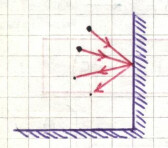
\includegraphics[scale=0.5]{images/1606329297.jpg}

Será
\[
	P = \int d^p 2 p_x v_x f_\text{eq}(\vbp)
\]
dado que la presión se relaciona con el flujo de momento.

Así llegamos a la función de Maxwell-Boltzmann
\[
	f_\text{eq}(\vbp) = \frac{ n }{( 2 \pi m k T )^{3/2}} \euler^{- (\vbp - \vbp_0)^2 / (2mkT)},
\]
que es la solución estacionaria de la ecuación de transporte de Boltzmann.
 
\end{ejemplo}

\begin{ejemplo}{\bf Problema 4 y comentario problema 6}

Ilustramos con

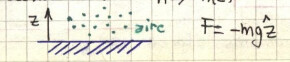
\includegraphics[scale=0.5]{images/1606329354.jpg}
 
\[
	\dpar{f}{t} + \frac{\vbp}{m} \dpar{f}{\vbx} + \frac{\vb{F}}{m}\dpar{f}{\vb{u}} =
	\left.\dpar{f}{t}\right|_\text{col} = 0,
\] 
en el campo gravitatorio terrestre, donde $\vb{F} = - m g z$ y entonces
\[
	\hat{z} v_x \dpar{f}{z} - g \hat{z} v_x \dpar{f}{v_z} = 0
\]
de modo que planteo 
\[
	f = \frac{ n(z) }{( 2 \pi m k T )^{3/2}} \euler^{- (\vbp - \vbp_0)^2 / (2mkT)}
\]
entonces, reemplazando, resulta en
\[
	\dtot{n(z)}{z} = - g \frac{m}{kT} n(z)
\]
y
\[
	n(z) = n_0 \euler^{-\beta m z g}.
\]
 
En el problema 6 se tiene una situación parecida 

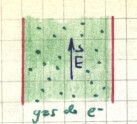
\includegraphics[scale=0.5]{images/1606329360.jpg}

pero aquí es $\vb{F} = - e E_0 \zver$ con la misma ecuación. No obstante cualitativamente la cosa cambia:
la simetría marca un piso en el problema anterior pero es indiferente (no hay ceros) en la situación del
campo eléctrico $\vb{E}$ puesto que hay simetría de traslación $ \nabla_x = 0$ (lejos de los bordes).
En el caso del campo gravitatorio no se desprecia $ \nabla_x $

\[
	\left( v_z \dpar{}{v_z} - m g \dpar{}{v_z} \right) f = \left.\dpar{f}{t}\right|_\text{col}
\]
y a orden cero,
\[
	\left( v_z \dpar{}{v_z} - m g \dpar{}{v_z} \right) f = 0,
\]
pero 
\[
	- \frac{eE_0}{m} \dpar{f}{v_z} = \left.\dpar{f}{t}\right|_\text{col}
\]
a orden cero da $\partial f / \partial v_z = 0 $ de manera que como el orden cero no tiene sentido hay que
ir al orden uno
\[
	- \frac{eE_0}{m} \dpar{f}{v_z} = - \frac{f_1}{\tau}.
\]
  
\end{ejemplo}



\subsection{Gas ideal (microcanónico)}

Esto es parte del problema 1 de la serie 4. Mixeo con este contenido.
El hamiltoniano que se considera es:
\[
	\Ham =  \sum_i^{N} \frac{p^2_i}{2m}
\]
y como $ 2 m E = \sum_i^N \: p_i^2 $ se puede pensar en una hiperesfera de radio $\sqrt{2mE}$.
\[
	\Sigma(E) = \frac{1}{h^{3N}} \int_{\Ham < E} d^3p_1 ... d^3p_N d^3q_1 ... d^3q_N = 
	\left( \frac{V}{h^{3N}} \right)^N \int_{\Ham < E} d^3p_1 ... d^3p_N
\]
donde la integral en $\{ q_i\}$ es inmediata porque no están los mismos en los límites y donde el
límite de integración $\Ham < E$ implica la condición 
\[
	p_1^2 + p_2^2 + ... + p_N^2 < ( \sqrt{2mE} )^2.
\]
Se ve que $\Sigma(E) $ será el volumen de la hiperesfera mientras que $\Gamma(E)$ sería su
superficie.

Se puede ver que 
\[
	\Sigma(E) = C_{3N} \Frac{V}{h^3}^N \Omega_{3N}( R = \sqrt{2mE} )
\]
donde $ \Omega $ es el volumen de la esfera $3N-$dimensional con radio $\sqrt{2mE}$.
Usamos para ello la fórmula del apéndice ALGO.

Volviendo al problema, tenemos
\[
	\Sigma(E) = C_{3N} \left[ \frac{V}{h^3} (2mE)^{3/2}\right]^N
\]
donde $C_{3N}= \pi^{3/2} / (3 N/2)! $.

Luego, tomando logaritmo resulta
\[
	\log \Sigma(E) = \log C_{3N} + N \log \frac{V}{h^3} + \frac{3N}{2} \log (2mE)
\]
y si se usa la aproximación de Stirling en el primer término (que contiene un logaritmo) 
se debería llegar, amasando un poco, a
\notamargen{Stirling: \[ \log(N!) = N\log N - N \]}

\[
	S(E,V) = N k \log \left[ V \Frac{4 \pi m E}{3 h^2 N}^{3/2} \right] + \frac{3}{2} Nk
\]
\[
	E(S,V) = \Frac{3h^2}{4\pi m} \frac{N}{V^{2/3}} \euler^{ 2/3(S/(Nk) -1 )}
\]

Consigno aquí abajo lo que tenía previamente (hay que consolidar)
\[
	S = k \log \left\{ C\left( \frac{V}{h^3}(2mE)^{3/2}\right)^N \right\}
\]
\[
	S = k \log C + N k \log \left[ \frac{V}{h^3}(2mE)^{3/2}\right]
\]
\notamargen{$ k\log C \approx -3/2 Nk \log 3N/2 $}

Calculando la temperatura desde aquí resulta en
\[
	\left. \dpar{S}{E} \right|_{V,N} = \frac{1}{T} \qquad \Rightarrow \qquad \frac{1}{T} = Nk\frac{3}{2}\frac{1}{E}
\]
y entonces
\[
	E = \frac{3}{2} NkT,
\]
que es la energía del gas ideal.
Entonces desde la mecánica estadística hemos llegado a la termodinámica. Recordemos que
\notamargen{Vemos que la termodinámica es bastante insensible a las aproximaciones.}
se tiene también
\[
	P = - \dpare{E}{V}{N,S} = \frac{2E}{3V} \qquad \qquad PV = NkT
\]
que conduce a lo mismo (lo cual sabemos de la infancia termodinámica).

El asunto es que la entropía $S$ a la cual hemos llegado no es aditiva. Esto, creo, sería la paradoja de Gibbs.

\subsection{Paradoja de Gibbs}

Tengo el sistemita de dos contenedores cada uno con $N_i, V_i$ ($i=1,2$) donde $N=N_1+N_2$ y $V=V_1+V_2$.
Si retiro el tabique se tiene $S_T > S_1 + S_2$ porque inicialmente estaban en equilibrio.
Quitar la pared es una operación mental si los gases son idénticos (o al menos eso podemos pensar).

Gibbs dice que hemos contado mal la $\Gamma(E)$ y plantea que considerando a manopla una
\[
	\Sigma'(E) = \frac{\Sigma(E)}{N!}
\]
porque las partículas son indistinguibles, reduciendo el número de microestados, se resuelve el tema y se
tiene una función $S$ aditiva.
El tema es que uno utiliza razonamientos clásicos con distinguibilidad entonces llegamos a un resultado
clásico.

\[
	S \propto Nk\log(V) + Nk \log (E^{3/2})
\]
Supongamos dos gases idénticos con la misma $\rho$ y $T$


\[
	\Delta S = Nk \log V + Nk \log (E^{3/2}) - N_1k \log V_1 - N_2k \log (E_1^{3/2})
	- N_1k \log V_2 - N_2k \log (E_2^{3/2})
\]
\[
	\Delta S = N_1 k \log \left( \frac{V}{V_1} \right) + N_2 k \log \left( \frac{V}{V_2} \right) +
		N_1 k \log \left( \frac{E}{E_1} \right)^{3/2} + N_2 k \log \left( \frac{E}{E_2} \right)^{3/2}
\]
\notamargen{Si los gases son distintos está correcto $\Delta S > 0$ pero si son idénticos no porque un estado
como F podría provenir de infinitas compartimentacionales las cuales darían todas difrentes $\Delta S$ y entonces
la entropía $S$ no sería función de estado.}
\[
	\Delta S > 0 \quad \text{pues: } \; \frac{V}{V_1} = 1 + \frac{V_2}{V_1} > 1, \frac{V}{V_2} > 1, 
	\frac{E}{E_1} > 1, \frac{E}{E_2} > 1
\]

Podemos hacer algo menos cuentoso tomando
\[
	S \propto Nk\log \left( V\left[ \frac{4\pi m E}{3 h^2 N} \right]^{3/2} \right)
\]
donde la $N$ viene de $k\log C_{3N}$ con $N \to \infty$. Vemos que $E/N$ mantiene el cambio en $S$ respecto de $E$
igual, puesto que 
\[
	\frac{E}{N} = \frac{E_1 + E_2}{N_1 + N_2} = \frac{E_1}{N_1} = \frac{E_2}{N_2} = \epsilon
\]
pero $V$ no balance. Luego la inclusión de $1/N!$ hará que 
\[
	S = k \log (\frac{1}{N!}\Sigma(E,N,V)) = k \log (\Sigma) - k\log N!
\]
de forma que resultará
\[
	S \propto Nk\log \left( \frac{V}{N}\left[ \frac{4\pi m E}{3 h^2 N} \right]^{3/2} \right)
\]
y esta $S$ sí está libre de paradoja de Gibbs.

\begin{ejemplo}{\bf Problema 3}

Considero $v = \lambda^3 $ con 
\[
	\lambda = \frac{\hbar}{\sqrt{2 m k T}}
\]
se toma distinguibilidad pero se puede hacer considerando indistinguibilidad.
 
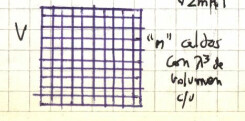
\includegraphics[scale=0.5]{images/1606329374.jpg} 

La cantidad de celdas es $n = N / \lambda^3$ y es un gas diluído $ N \ll n $ de manera en que
$\Gamma$ es el número de estados posibles del sistema, o bien el número de maneras de ubicar
$N$ partículas en $n$ celdas.
 
\end{ejemplo}



% =================================================================================================
\section{Ensamble canónico}
% =================================================================================================

Consideramos un microcanónico con 
\[
	E = E_1 + E_2, \qquad N = N_1 + N_2, \qquad V = V_1 + V_2 
\]
donde $N_i, V_i$ están fijos y $E_i$ varían de acuerdo a
\[
	E = E_1 + E_2
\]

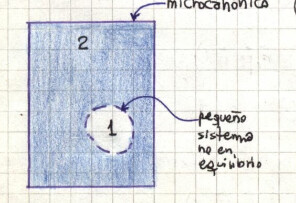
\includegraphics[scale=0.5]{images/1606329302.jpg}

La idea es que el sistema 2 es tan grande como se quiera y el sistema 1 es pequeño pero macroscópico;
entonces el primero actúa como un baño térmico, un reservorio de calor que le fijará la temperatura $T$.
O sea que será un problema isotérmico.


Consideramos un microcanónico 
\[
	\Gamma(E) = \Sigma_{E_1} \Gamma_1(E_1) \Gamma_2(E-E_1) \leq C \Gamma_1(\bar{E}_1) \Gamma_2(E-\bar{E}_1)
	\approx C \Gamma_2(\bar{E}_1)
\]
\[
	S(E-\bar{E}_1) \approx k \log \Gamma_2(E-\bar{E}_1)
\]
\[
	S(E) + \left.\dpar{S(E)}{E}\right|_E(-\bar{E}_1) \approx k \log \Gamma_2(E-\bar{E}_1)
\]
\[
	\euler^{\frac{S(E)}{k}} \euler^{-\frac{E_1}{kT}} \approx \Gamma_2(E-\bar{E}_1)
\]

Claramente como '1' siempre está metido dentro de '2' entre mayor sea el $\Gamma_2$ mayor también el tamaño de '1'
en $\mathbb{\Gamma}$, luego:
\[
	\# \text{de config en } \mathbb{\Gamma} \text{ del sistema '1+2'} = \# \text{de config de '1' en '2'} \times 
	\# \text{de config de '2' en} \mathbb{\Gamma}
\]
\[
	\# \text{ config '1' } = \frac{ \# \text{ config '1+2'} }{ \# \text{ config '2'} } \approx 
	\euler^{-\frac{E_1}{kT}} = C \int \euler^{-\Ham/kT} d^3p d^3q
\]
y se integra para toda energía
\[
	Q_N(V,T) = \frac{1}{h^{3N}N!}\int \euler^{-\Ham/kT} d^3p d^3q
\]
\notamargen{$1/N!$ es el factor de buen conteo.}

{\bf comentarios sobre ensambles}

O sea que ahora densidad de estados tiene forma $\euler^{-\frac{E_1}{kT}}$ y la función de partición
$Z(V,T,N)$ que está arriba, que sería el volumen ocupado en el espacio de fases con la corrección
del factor de buen conteo.

\notamargen{¿$\lambda^3$ es igual a $h^3$?}

En el microcanónico $E$ es constante, pero en el canónico no. Los valores medios deberían ser parecidos
porque el pequeño es una parte del todo.
Las dos cosas convergeán al mismo valor. Veamos un argumento de plausibilidad.
\[
	Z_C = \int_0^\infty \: dE \omega(E) \euler^{-\beta E}
\]
donde $\omega(E)$ es la densidad de estados de energía entre $(E,E+dE)$. Ésta será función creciente
porque a mayor enegrgía más degeneración.

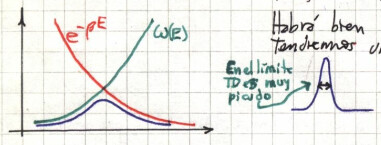
\includegraphics[scale=0.5]{images/1606329392.jpg}

Existirá un valor bien definido $\vm{E}$ para el canónico tendremos una distribución.

En el canónico todos los puntos participan, aunque los que realmente aportan son los que están en torno
al valor medio.
\[
	Z_C = \int dE \euler^{-\beta E + \log \omega(E)} =
	\int dE \euler^{-\beta ( E - TS(E)) }
\]
y buscaré máximo del argumento de la exponencial ($E$ mínima y $S$ máxima). Con $T$ chica minimizo $E$ y
con $T$ grande maximizo $S$.
Las funciones $S,E$ van como $N$ y la única parte que contribuye es la que tiene el argumento máximo.

La energía en el canónico no es constante pero aproximadamente $ \vm{E} = \vm{E}(T) $. En el microcanónico
hago una cuenta $(E,V,N)$  y para el canónico puedo tomar una $T$ que haga que $ \vm{E}(T) \sim E$.

{\bf fin del interludio}

Los microestados no son equiprobables, hay una distribución de probabilidad, que normalizada es
\[
	P_{\mu-\text{estado}} = \frac{ \euler^{-\beta E_{\mu e}} }{ \displaystyle \sum_{\mu e} \euler^{-\beta E_{\mu e}} }
\]

La función de partición es el volumen ocupado en $\mathbb{\Gamma}$. En el caso discreto es
\[
	Z_c(N) = Q_N(V,T) = \sum_{\mu e} \frac{1}{N!} \euler^{-\beta E_{\mu e}}
\]
mientras que en el continuo es la expresión de arriba.


El vínculo con la termodinámica viene de
\[
	Q_N(V,T) = \euler^{-\beta A}
\]
\[
	A = -kT\log [Q_N(V,T)] \qquad \qquad A = U - TS
\]
\[
	P = -\dpare{A}{V}{T} \qquad \qquad S = -\dpare{A}{T}{V}
\]
donde $A=A(T,V,N)$ es la energía libre de Helmholtz. Podemos ver que se deduce esto de 
\[
	< \Ham > = E = -\dpar{}{\beta} \log [ Q_N(V,T) ] = A + TS = A - T\left.\dpar{A}{T}\right|_{N,V}
\]
pero 
\[
	\dpar{}{\beta} = \dpar{}{T} \dpar{T}{\beta} = -k T^2 \dpar{}{T}, \qquad \text{pues } \dpar{\beta}{T} = - 
	\frac{1}{kT^2}
\]
\[
	\dpar{}{T}\left( \frac{A}{T} \right) = -\frac{A}{T^2} + \frac{1}{T}\dpar{A}{T}
\]
de modo que 
\[
	-T^2 \dpar{}{T}\left( \frac{A}{T} \right) = A - T \dpar{A}{T}
\]
\notamargen{$S=-\partial A / \partial T|_{N,V}$}
y entonces
\[
	E = -k T^2 \dpar{}{T}\log Q_N = -T^2 \dpar{}{T}\left( \frac{A}{T} \right) 
\]
de lo que se desprende
\[
	\log Q_N = -\frac{A}{kT}
\]

Podemos usar $E=A+TS$ y llegar a $Q_n=\exp(-\beta A)$ o bien $Q_N=exp(-\beta A)$ y llegar a $E=A+TS$.

\subsection{Equivalencia canónico y microcanónico}

Vemos cómo son las fluctuaciones de energía en el canónico. Desde 
\[
	U = <\Ham> = \frac{\int \euler^{-\beta\Ham} \Ham d^3p d^3q}{\int \euler^{-\beta\Ham} d^3p d^3q}
\]
\[
	\int \euler^{-\beta\Ham} U d^3p d^3q = \int \euler^{-\beta\Ham} \Ham d^3p d^3q
\]
\[
	\dpar{}{\beta}\left[ \int \euler^{-\beta\Ham} (U-\Ham) d^3p d^3q\right] = \dpar{}{\beta}\left[ 0 \right] = 0
\]
\[
	<\Ham^2> - <\Ham>^2 = kT^2C_V
\]

Las fluctuaciones van como el $C_V$, luego 
\[
	<\Ham^2/N^2> - <\Ham/N>^2 = kT^2c_V/N \qquad \text{donde } c_V = C_V/N
\]
\notamargen{$<\Ham> \propto N$ y $C_V \propto N$}
de modo que las fluctuaciones relativas van a 0 con $N\to\infty$.

Otro modo de verlo es considerando 
\[
	\frac{1}{h^{3N}N!}\int \euler^{-\beta\Ham} d^3p d^3q = \int_0^\infty dE \dpar{\Sigma(E)}{E} \euler^{-\beta E} =
	\int_0^\infty dE \euler^{-\beta E + \log (\partial \Sigma(E)/\partial E)}
\]
donde 
\[
	\dpar{\Sigma(E)}{E} dE = \frac{d^3p d^3q}{h^{3N}N!}
\]
y como $S/k = \beta TS$
\[
	Q_N = \int_0^\infty dE \euler^{-\beta E + \beta T S }
\]

Si suponemos que es $S$ máxima en $E=\bar{E}$ entonces $S_{MAX} = S(\bar{E})$ y será 
\[
	\left. \dpar{S}{E} \right|_{\bar{E}} = 0
\]
con lo cual
\[
	E + TS \cong \bar{E} + TS(\bar{E}) + \frac{1}{2}(E-\bar{E})^2 T \left. \dpar[2]{S}{E} \right|_{\bar{E}}
\]
\[
	E + TS \cong \bar{E} + TS(\bar{E}) - (E-\bar{E})^2 \frac{1}{2kTC_V}
\]
de modo que 
\[
	Q_N = \int_0^\infty dE \euler^{-\beta [\bar{E} + TS(\bar{E})] - \beta \frac{(E-\bar{E})^2}{2kTC_V}}
\]
\[
	Q_N = \euler^{-\beta [\bar{E} + TS(\bar{E})]} \int_0^\infty dE \euler^{- \beta \frac{(E-\bar{E})^2}{2kTC_V}}
\]
y vemos que la integral se va a una delta con $N\to \infty$ (pués $C_V \propto N$) en cuyo caso
\[
	Q_N = \euler^{-\beta [\bar{E} + TS(\bar{E})]} 
\]
y la mayor parte de los estados tienen energía $\bar{E}$, que es la de un sistema aislado a temperatura $T$.

La densidad de estados va entonces de acuerdo al producto de dos efectos contrarios:
\[
	g(E) = \dpar{\Sigma(E)}{E}\euler^{-\beta E}
\]

\subsection{Ejemplos sencillos}

\[
	\Ham = \sum_i^N \frac{p_i^2}{2m} + \frac{m}{2}\omega_i^2 q_i^2 \quad \qquad \text{oscilador clásico 1D}
\]
\[
	\Ham = \sum_i^N \left( n_i + \frac{1}{2} \right)\hbar\omega  \quad \qquad \text{oscilador Schrödinger 1D}
\]
\[
	\Ham = \sum_i^N  n_i \hbar\omega \quad \qquad \text{oscilador Planck 1D}
\]

\[
	U = NkT \rightarrow C_V = Nk  \qquad \text{Clásico}
\]
\[
	U \approx \frac{N\hbar\omega}{2} \quad U \approx 0 (T\ll 1) \qquad \rightarrow C_V = 0 
	\quad \text{Schrödinger-Planck}
\]
\[
	U \approx N kT \; (T \gg 1) \qquad \rightarrow C_V = Nk 
	\quad \text{Schrödinger-Planck}
\]

Los casos Schrödinger y Planck aproximan al $C_V$ clásico con $T$ altas.

\begin{ejemplo}{\bf Problema 1 (serie 5)}

(a) Tenemos un oscilador armónico en un baño a temperatura $T$
\[
	E_n = \left( n + \frac 1 2 \right) \hbar \omega 
\]
donde
\[
	\frac {k T} { \hbar \omega } \ll 1
\]
que implica que la energía que le da el baño es pequeña, y donde el ratio es entre la energía media
que cede o entrega la fuenta y el cuanto de energia del oscilador armónico.

La función de partición será
\[
	Z_C = \sum_n^\infty  \: \euler^{ - \beta E_n } =  \sum_n^\infty  \: \euler^{ - \beta (n+1/2) \hbar\omega }
\]
que se puede trabajar como
\[
	Z_C = \euler^{ - \beta\hbar\omega/2 } \sum_n^\infty  \: \euler^{ - \beta n \hbar\omega }
	= \euler^{ - \beta\hbar\omega/2 } \frac{1}{ 1 -\euler^{ - \beta \hbar\omega } }
\]
donde hemos usado la suma geométrica. Luego aproximando
\[
	Z_C = \frac{1}{ \euler^{ \beta \hbar\omega /2 } - \euler^{ - \beta \hbar\omega/2 } } \approx 
	\euler^{ - \beta \hbar\omega /2 }
\]
Entonces, el cociente
\[
	\frac{P(n=1)}{P(n=0)} = \euler^{ - \beta \hbar\omega } = \euler^{ - \beta \Delta E }
\]
de manera que a $T$ mayor crece la probabilidad. La probabilidad de la relación entre $ \beta $ y $\hbar \omega$.


(b) El valor medio de la energía será
\[
	\vm{E} = P (n=0) \frac{\hbar \omega}{2} + P(n=1)\frac{3\hbar \omega}{2} + ...
\]
que aproximadamente es
\[
	\frac{\hbar \omega}{2Z_C}  \euler^{ - \beta \hbar\omega/2 } 
	\left( 1 +  3 \euler^{ -\beta\hbar\omega/2 } \right)
\]

\[
	\vm{E} = \frac{}{×}  \euler^{ - \beta \hbar\omega/2 } \frac{ 1 + 3 \euler^{-\beta \hbar}}
	{\euler^{ \beta \hbar\omega /2 } - \euler^{ - \beta \hbar\omega/2 }  } = \frac{\hbar \omega }{2}
	\left[ \frac{1 + 3 \euler^{ -\beta\hbar\omega } }{ 1 + \euler^{ -\beta\hbar\omega } } \right]
\]
En esta cuenta me quedo al mismo orden en $Z_C$.
En realidad no se plancha, sino que por haber aproximado a dos niveles tenglo el límite.
Entonces en esta zona voldraá bien el cálculo hecho.

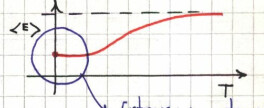
\includegraphics[scale=0.5]{images/1606329403.jpg} 

 
\end{ejemplo}

\begin{ejemplo}{\bf Problema 2}
 
\end{ejemplo}

\begin{ejemplo}{\bf Problema 3}
 
\end{ejemplo}

\subsection{Una derivación más del canónico}

El tamaño del sistema '1' en $\mathbb{\Gamma}$ (su volumen $\Gamma_1(E_1)$) será proporcional al tamaño del sistema 
'2' en $\mathbb{\Gamma}$ (su volumen $\Gamma_2(E-E_1)$) de manera que 
\[
	\Gamma_1(E_1) \propto \Gamma_2(E-E_1)
\]
\[
	k\log \Gamma_1(E_1) \approx S(E) + \left.\dpar{S}{E}\right|_E (-E_1) = S(E) - \frac{E_1}{T} 
	\text{ (del sistema '2') }
\]
\[
	\Gamma_1(E_1) \approx \euler^{S(E)/k} \euler^{-E_1/kT} 
\]
\[
	\text{ \# conf '1' } = \text{ \# conf '2' } \times \text{ densidad del '1' en el '2' }
\]
y finalmente
\[
	Q_N (V,T) = \frac{1}{h^{3N}N!} \int d^{3N}p d^{3N}q \euler^{-\Ham(\{ p_i,q_i\})/kT}
\]

% =================================================================================================
\section{Líquidos}
% =================================================================================================

En un gas real se tiene
\[
	H = \sum_i^N \frac{p_i^2}{2m} + \sum_{i<j} V_{ij}
\]
\[
	Z_N = \int d^{3N}q \: \euler^{ - \beta \sum_{i<j} V_{ij} },
\]
que es la integral configuracional; acá está la parte jodida porque están acopladas las coordenadas.

La expresión del virial no sirve en la región de la transición de fase.
A orden uno se obtiene la densidad,
\[
	\frac{1}{V} \int dq = \frac{N}{V} = \rho 
\]

Esto es la probabilidad de hallar una partícula en $r_1$. Si hay dos partículas ya no es $\rho^2$ porque
están interactuando. Hay una función de correlación $g^2(r_1,r_2)$ que se puede determinar experimentalmente.

\notamargen{En el límite de un cristal se tiene una sucesión de deltas picudas}

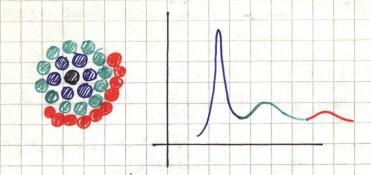
\includegraphics[scale=0.5]{images/1606329384.jpg} 

Podemos hallar $g(r)$ y su relación con la termodinámica. Asumimos que tenemos $g(r), g(r)^2$ es la función
de correlación de cuerpos.

$\xi$ prende o apaga la partícula 1.

Con $N$ muy grande (variando de a uno): calcular $\mu$ es \textit{encender} o \textit{apagar} una partícula.

\subsection{Comentarios problemas ensambles}

% =================================================================================================
\section{El gran canónico}
% =================================================================================================

La desventaja del microcanónico es la de tener que calcular todos los estados accesibles.
El canónino es un subconjunto del microcanónico.

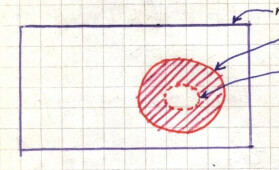
\includegraphics[scale=0.5]{images/1606329345.jpg} 
La caja es un microcanónico, el rojo es un canónico donde está fija la temperatura $T$ y el
conjuntillo más interno es una pared porosa que lo limita.

El $1/N!$ corrige la indistinguibilidad de las partículas -es el factor de buen conteo de Boltzmann-.
Se define la fugacidad $ z \equiv \euler^{ \beta \mu } $.

Para un sistema con un número de partículas determinadas puedo utilizar el GC que será más sencillo
que el MC o el C. La densidad o el número medio de partículas es algo que fijo desde fuera; el número
de partículas fluctuará y querremos calcular dicha fluctuación (que se hace en la próxima
subsección).

Todos los ensambles son equivalentes si $N \to \infty$. De lo contrario, con $N$ no infinito
tendríamos tres termodinámicas diferentes dadas por el microcanónico, el canónico y el gran canónico.
Cuando calculamos la fluctuación de energía surge una parte asociada a la variación del número de
partículas. $\partial p / \partial v = 0$ ocurre en particular en la región de coexistencia.

Se asume que el sistema satisface
\begin{itemize}
 \item Potencial tipo carozo duro + cola finita. Dado un volumen $V$ existe $N$ máximo.
 \item \[
	A(N,V) = - \frac{V}{\beta} f(\nu)
 \]
 escalea con el volumen.
 \item Como $f(\nu)$ satisface $ \partial p / \partial v \leq 0$ entonces ...
\end{itemize}

Se obtiene una función de potencial GC $\Xi$ que debe ser un polinomio en $N$ de grado 
$N_0(V) = a V$ para $V$ grande.


\[
	Q_N (V,T) =  \frac{1}{h^{3N}N!} \int d^{3N_1}p_1 d^{3N_2}p_2  \sum_{N_1=0}^N \frac{N!}{N_1! N_2!}
	\int d^{3N_1}q_1 d^{3N_2}q_2 \euler^{-\beta [\Ham_1 + \Ham_2 ]}
\]
\[
	Q_N (V,T) =  \frac{1}{h^{3N_1} h^{3N_2} } \sum_{N_1=0}^N \frac{1}{N_1! N_2!}
	\int d^{3N_1}p_1 d^{3N_1}p_1 \euler^{-\beta\Ham_1} \int d^{3N_2}q_2 d^{3N_2}q_2 \euler^{-\beta\Ham_2}
\]
\[
	Q_N (V,T) =  \sum_{N_1=0}^N \int \frac{1}{h^{3N_1}N_1!} d^{3N_1}p_1 d^{3N_1}p_1 \euler^{-\beta \Ham_1 }
	\int \frac{1}{h^{3N_2}N_2!} d^{3N_2}q_2 d^{3N_2}q_2 \euler^{-\beta \Ham_2 }
\]
\[
	1 = 
	\sum_{N_1=0}^N \frac{1}{h^{3N_1}N_1!} \int d^{3N_1}q_1 d^{3N_1}p_1 \; 
	\euler^{-\beta\Ham_1} \frac{Q_{N_2}(V_2,T)}{Q_N(V,T)} 
\]
\[
	1 = 
	\sum_{N_1=0}^N \int d^{3N_1}q_1 d^{3N_1}p_1 \; \frac{\euler^{-\beta\Ham_1}}{h^{3N_1}N_1!} 
	\frac{Q_{N_2}(V_2,T)}{Q_N(V,T)} 
\]
siendo el último factor un $ \rho(\{ p_1,q_1\},N_1)$
\[
	\frac{Q_{N_2}(V_2,T)}{Q_N(V,T)} = \euler^{-\beta A (V-V_1,N-N_1,T)}\euler^{-\beta A (V,N,T)} =
	\euler^{-\beta [ \frac{\delta A}{\delta V} \delta V + \frac{\delta A}{\delta N} \delta N ] }
\]
donde las diferencias $\delta$ se toman discretas:
\[
	\frac{\delta A}{\delta V} \delta V + \frac{\delta A}{\delta N} \delta N =
	(-p )(-V_1) + \mu (-N)_1 = pV_1 - \mu N_1
\]
\[
	A = U - TS \qquad dA = dU - TdS - SdT = -pdV + \mu dN - SdT
\]
\[
	\frac{Q_{N_2}(V_2,T)}{Q_N(V,T)} = \euler^{-\beta PV_1 + \beta \mu N_1},
\]

De forma que la densidad del sistema '1' es
\[
	\frac{1}{h^{3N_1}N_1!} \euler^{-\beta\Ham_1}  \euler^{-\beta PV_1}  \euler^{\beta \mu N},
\]
y definiendo $z \equiv \euler^{\beta\mu}$
\[
	\rho(\{p,q\},N) = \frac{z^N}{h^{3N}N!} \euler^{-\beta\Ham}  \euler^{-\beta PV} 
\]

Nótese que $ \mu, P, V, T$  son los valores fijos del sistema mayor y hemos sacado subíndices.
\[
	1 = \sum_{N=0}^\infty \int d^{3N}q d^{3N}p \frac{z^N}{h^{3N}N!} \euler^{-\beta\Ham}  \euler^{-\beta PV} 
\]
\[
	\euler^{\beta PV} = \sum_{N=0}^\infty \frac{z^N}{h^{3N}N!} \int d^{3N}q d^{3N}p \euler^{-\beta\Ham}
	= \sum_{N=0}^\infty z^N Q_N(V,T)
\]
\be
	\beta PV = \log \left( \sum_{N=0}^\infty z^N Q_N(V,T) \right)
	\label{betaPV}
\ee
y tenemos 
\[
	\Xi(z,V,T) \equiv \sum_{N=0}^\infty z^N Q_N(V,T)
\]
que es la gran función de partición.
La termodinámica puede extraerse desde 
\[
	<N> = z\dpar{}{z} \log [ \:\Xi(z,V,T) \:]     \qquad 
	<E> = -\dpar{}{\beta} \log [ \:\Xi(z,V,T)\: ]
\]

La ecuación de estado se obtiene reemplazando $z$ en la expresión de \eqref{betaPV} y en $<N>$


\subsection{Fluctuaciones de densidad}

\[
	<N^2> - <N>^2 =  z\dpar{}{z}\left( z\dpar{}{z} \log \Xi \right)= kTV \dpar[2]{P}{\mu}
\]
\[
	<N^2> - <N>^2 = kTV \dpar{}{\mu}\frac{1}{v} = kTV \frac{1}{v^2}\kappa_T = kT\frac{N^2}{V}\kappa_T 
	= NkT \frac{\kappa_T}{v}
\]
\notamargen{Viene de $\dpar{}{\mu}\frac{1}{v} = -\frac{1}{v^2} \frac{1}{v} \dpar{v}{P} = \frac{1}{v^2}\kappa_T $}

Si $A=Na$ entonces $a=u-Ts$ y entonces 
\[
	\dpar{a}{v} = -p
\]
\[
	U = TS-pV+\mu N \quad \Rightarrow \quad u = Ts - pv
\]
\[
	\dpar{\mu}{v} = -P -v\dpar[2]{a}{v} + p = v \dpar{p}{v} \qquad \dpar{p}{\mu} \qquad 
			= \frac{\dpar{p}{v}}{\dpar{\mu}{v}}=\frac{1}{v}
\]
pues 
\[
	u - Ts = a = - pV + \mu \qquad \mu = a + pv
\]

Las fluctuaciones relativas tiende a cero cuando $N\to\infty$ provistos de que $\kappa_T < \infty$. Esto no vale 
en la transición de fase de primer oden pues 
\[
	\left. \dpar{p}{v} \right|_{\text{punto crítico}} = 0 \qquad \frac{1}{v} \dpar{v}{p} \to \infty
\]
Se calculan como 
\[
	\sqrt{\frac{<N^2> - <N>^2}{N^2}} = \sqrt{ kT\dpar{\kappa_T}{v}\frac{1}{N}} \to 0 \text{ si } N\to\infty
\]

\subsection{Fluctuaciones de energía}

\[
	<\Ham^2> - <\Ham>^2 = kT^2 \left( \dpar{U}{T} \right)_{z,V}
\]
y como 
\[
	\left( \dpar{U}{T} \right)_{z,V} = \left.\dpar{U}{T}\right|_{N,V} + \left.\dpar{U}{N}\right|_{T,V} 
	\left.\dpar{N}{T}\right|_{z,V}
\]
\[
	<\Ham^2> - <\Ham>^2 = kT^2C_V +  \left[\left. \dpar{U}{N} \right|_{T,V}\right]^2 <(\Delta N)^2>
\]
siendo $ kT^2C_V $ fluctuación del canónico y $(\Delta N)^2 = <N^2> - <N>^2 $

Si se considera la densidad
\[
	< h^2 > - < h >^2 = kT^2 \frac{k T^2 C_V}{N}, 
\]
y con $ N \to \infty $ estas fluctuaciones de energía se van a cero.

Para un problema de estas características puedo elegir canónico o microcanónico; los ensambles son
indistinguibles de modo que son equivalentes. En cambio, si $N$ es grande no son equivalentes.

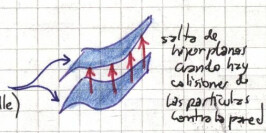
\includegraphics[scale=0.5]{images/1606329307.jpg} 
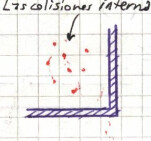
\includegraphics[scale=0.5]{images/1606329311.jpg}

Los de la izquierda son hiperplanos en $\Gamma$ (satisface Liouville); las colisiones internas (derecha)
generan movimiento en cada hiperplano que representa un volumen en $\Gamma$.
La densidad de estados $\rho$ decae exponencialmente. Tenemos dos fenómenos contrarios:
el decaimiento de $\rho$ y el crecimiento del número de estados a una energía

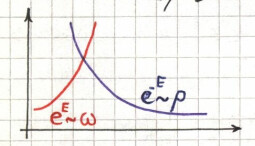
\includegraphics[scale=0.5]{images/1606329317.jpg}

Consideremos dipolos en campo magnético

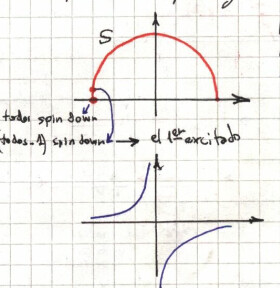
\includegraphics[scale=0.5]{images/1606329322.jpg}

La simetría de los dipolos up y down nos da la forma simétrica de la entropía $S$

Para las temperaturas tengo $T<0$ lo cual no puede medirse. No puedo medir con un termómetro; que
tiene un espectro continuo acotado.


\subsection{Gas ideal}

\[
	Q_N = \frac{(Vf(T))^N}{N!} \Rightarrow \Xi = \sum_{N=0}^\infty \frac{(zVf(t))^N}{N!} = \euler^{zVf(T)}
\]
\[
	\beta pV = \log (\Xi) = zVf(T) \qquad <N> = z \dpar{}{z} \log (\Xi) = zVf(T)
\]
y luego 
\[
	\beta pV = <N> \qquad \rightarrow \quad pV = <N> k T
\]
y recuperamos la ecuación de estado del gas ideal.


\subsection{Equivalencia canónico-gran canónico}

Para ver que con $ N \to \infty $ son equivalentes consideramos 
\[
	\kappa_T = \frac{1}{v} \left( -\dpar{v}{p} \right) < \infty \qquad \dpar{p}{v} < 0
\]

Pero en la coexistencia de una transición de fase de 1er orden se da 
\[
	\dpar{p}{v} = 0  \rightarrow \kappa_T \to \infty \text{ (sistema homogéneo) }
\]

La idea es ver que 
\begin{itemize}
 \item Dado $z$ existe $N$ tal que $ \Xi = \sum_N z^N Q_N(V,T) $
 \item Dado $N$ existe $z$ tal que $ \Xi = \sum_N z^N Q_N(V,T) $
\end{itemize}

Esto se comprueba. Además, si:
\[
	W (N) = z^N Q_N (V,T) \propto \text{ Prob. de que el sistema tenga $N$ partículas }
\]

XXX dibujos XXXX

En la transición de fase, donde $ \dpar{p}{v} = 0  $ todos los $ N $ son igual de probables porque
fluctúa la densidad. La $p$ se mantiene constante pero se varían los $ N_i $ de cada fase 'i'.


\subsection{Otra derivación del gran canónico}

Podemos derivar el gran canónico desde 
\notamargen{Es la probabilidad de hallar al sistema '1' en un estado con $ E_1, N_1 $.}
\[
	\text{Prob } \propto \Gamma_2(E-E_1, N-N_1)
\]
\[
	\log  \Gamma_2(E-E_1, N-N_1) \cong  \log \Gamma_2( E, N ) + \frac{1}{k} \left. \dpar{S(E,N)}{E} \right|_E(-E_1)
	+\frac{1}{k} \left. \dpar{S(E,N)}{N} \right|_N(-N_1)
\]
\[
	\cong \log \Gamma_2( E, N ) - \frac{E_1}{kT} + \frac{N_1\mu}{kT}
\]
\[
	\text{Prob } \propto \euler^{-\beta E}  \euler^{\beta \mu N}  = \euler^{-\beta E} z^N
\]
donde $T$ y $\mu$ son las asociadas al baño.
\notamargen{$\partial S/\partial E = 1/T$ y $\partial S/\partial N = -\mu / T$.}

Pensamos en $\eta$ copias del sistema; $n_{E_1N_1} = \# $ de sistemas con energía $E_1$ y $N_1$ partículas,
luego 
\[
	\sum_{\{ E_1, N_1 \}} n_{E_1N_1} = \eta \qquad \sum_{\{ E_1, N_1 \}} n_{E_1N_1}E_1 = n\bar{E}_1 \cong 
	\text{ Energía Total }
\]
\[
	\sum_{\{ E_1, N_1 \}} n_{E_1N_1} N_1 = \eta \bar{N}_1 \cong \text{ \# Total de partículas (no físico) }
\]
donde $ \bar{N}_1 $ es el número de medio.
\[
	\Omega\{ n_{E_1N_1} \} = \frac{\eta !}{\prod (n_{E_1N_1})!} \qquad \text{ combinatorio }
\]

La conbinación de mayor volumen será 
\[
	\log \Omega - \alpha \sum n E_1 - \beta_L \sum n N_1 = 0
\]
\[
	-\sum \left[ n\log n - n - \alpha n E_1 - \beta_L n N_1 \right] = 0
\]
\[
	-\sum n \left[ \log n - 1 - \alpha E_1 - \beta_L N_1 \right] = 0 
	\rightarrow \log(\tilde{n}) = 1 + \alpha E_1 + \beta_L N_1
\]
\[
	\tilde{n} \propto \euler^{\alpha E_1 + \beta_L N_1}
\]
que es el conjunto $n_{E_1N_1}$ de mayor volumen en $ \Omega $.

Esperaremos qeu con $ \eta\to\infty $ sea $<n_{E_1N_1}> \cong \tilde{n}_{E_1N_1} $.
Para determinar $\alpha, \beta$ usaremos 
\[
	\tilde{N} \cong <N> = \dpar{}{\beta_L}\left( \log \sum_{\{ E_1, N_1 \}} 
	\euler^{\alpha E_1 + \beta_L N_1} \right)
\]
\[
	\tilde{E} \cong <\Ham> =  \dpar{}{\alpha}\left( \log \sum_{\{ E_1, N_1 \}}
	\euler^{\alpha E_1 + \beta_L N_1} \right)
\]

% =================================================================================================
\section{Entropía de Gibbs}
% =================================================================================================

Sea $X$ extensiva mecánica,
\[
	S = k \log \Gamma (E,X) \qquad dU = TdS + Y dX, \; \frac{dS}{k} = \beta dU + \xi dX
\]
\notamargen{Donde $\beta Y = \xi $}
Consideramos un sistema en equilibrio donde fluctúan $E$ y $X$ (sistema en contacto con reservorios)

Refiriéndo al estado $ \nu $
\[
	P_\nu = \frac{ \euler^{-\beta E_\nu - \xi X_\nu } }{ \sum_\nu \euler^{-\beta E_\nu - \xi X_\nu } } =
	\frac{ \euler^{-\beta E_\nu - \xi X_\nu }}{\Theta}
\]
\[
	<E> = -\dpar{}{\beta} \log \Theta  \qquad <X> = -\dpar{}{\xi} \log \Theta 
\]
\notamargen{Caso $X=N$ $z\dpar{}{z} \cong \dpar{}{\beta \mu }$ }
\[
	d( \log \Theta ) = -<E> d\beta - <X> d\xi 
\]

Sea 
\[
	\Lag \equiv -k \sum_\nu P_\nu \log P_\nu =
	-k \sum_\nu P_\nu \log \left[ \euler^{-\beta E_\nu - \xi X_\nu } \Theta^{-1} \right]
\]
\[
	\Lag = \sum_\nu P_\nu k \log \Theta + k P_\nu \beta E_\nu + k P_\nu \xi X_\nu
\]
\[
	\Lag = k\log \Theta + k\beta <E> + k\xi <X>
\]
\[
	d\Lag = k\beta d<E> + k\xi d<X>
\]

Es una transformada de Legendre que toma $\log \Theta$ y la lleva a una función de $ <E>, <X> $
\[
	d\Lag = k \beta dE + k \beta Y dX = dS = \frac{1}{T}dE + \frac{Y}{T} dX 
\]
entonces $\Lag$ es la entropía $S$ (parecida al H de Boltzmann[?]).
\[
	\Lag = -k \sum_\nu P_\nu \log P_\nu 
\]
y $\nu$ son equiprobables
\[
	\Lag = -k \sum_\nu \frac{1}{\Gamma} \log \left( \frac{1}{\Gamma} \right) = 
	\sum_\nu \frac{k}{\Gamma} \log(\Gamma)
\]
y entonces
\[
	\Lag = k \log( \Gamma ) \equiv S.
\]

La entropía de Gibbs se reduce a la entropía de Boltzmann cuando los estados son equiprobables.

\begin{itemize}
 \item Microcanónico: requiere que ``cuente'' todos los estados.
 \item Canónico: me quito de encima la condición sobre la $E$.
 \item Gran canónico: me sacao de encima la condición sobre el número de partículas.
\end{itemize}

Pero las fluctuaciones de $E$ y $N$ van a cero con $N \to \infty$ y son equivalentes.


\subsection{Observación promedios}

\[
	<G> = \frac{\sum_N z^N G Q_N(V,T) }{\Xi} = \frac{\sum_N z^N \sum_\nu G(E_\nu, N, T) Q_N(V,T) }{\Xi}
\]
donde el último factor en la sumatoria es $<G>_{\text{CAN}} Q_N(V,T)$.

La parte crítica está en el pasaje de 
\[
	\sum_\nu \euler^{ -\beta E_\nu }
\]
a algún índice útil que permite realizar la sumatoria. En el caso de cuasipartículas, como osciladores, 
tenemos
\[
	\hat{H} = \sum_i^N \left( n_i + \frac{1}{2} \right) \hbar \omega_i 
\]
donde $ n_i $ es el número de fotones del oscilador i-ésimo. Los fonones cumplen el rol de partículas
\footnote{Porque podemos considerar que la $\sum$ se hace en niveles energéticos en lugar de entre osciladores
y tenemos un \# indeterminado de ``particulas'' (fonones) distribuidas en 'N' niveles energéticos.}
Un oscilador ddado puede tener en principio cualquier valor de energía (cualquier valor de $ n_i $) y esto 
independientemente de los otros $ N-1 $ osciladores. El número total de fonones del sistema
\[
	\sum_i^N n_i
\]
no es una constante del mismo con lo cual no hay vínculo. Entonces
\[
	\sum_\nu \qquad \rightarrow \qquad \sum_{n_1=0}^\infty \sum_{n_2=0}^\infty ... \sum_{n_\nu=0}^\infty
\]


\section{SUELTO: reubicar}

\[
	Z_N = \int d^{3N}q \prod_{i<j}^N (1+f_{ij}) \qquad \text{ integral configuracional }
\]
En realidad esta integral serán $ N(N-1)/2 $ integrales (N-grafos). Podemos factorizar los $ N(N-1)/2 $ grafos
en l-racimos teniendo en cuenta que se cumple
\[
	N = \sum_{l=1}^N ln_l,
\]
de forma que cada N-grafo dtermina un conjunto $ \{ m_l \} = (m_1,m_2, ..., m_N) $ de '$m_1$' 1-racimos, '$m_2$' 
2-racimos y '$m_N$' N-racimos. Por supuesto, un mismo conjunto $ \{ m_l \} $ determina muchos (en principio) N-grafos 
en función de la permutación de etiquetas.
\[
	\frac{N(N-1)}{2} \text{ N-grafos } \rightarrow M \text{ conjuntos } \{ m_l \}
\]
y la 
\[
	Z_N = \sum_1^{N(N-1)/2 } \text{ N-grafos } \quad \equiv \quad \sum_ {\{ m_l \}}' S(\{ m_l \})
\]
donde 
\[
	S(\{ m_l \}) = \prod_{l=1}^N \left( \sum \text{ l-racimos de l partículas }\right)^{m_l}
	\frac{N!}{ 1!^{m_1} 2!^{m_2} ..,N!^{m_N} m_1! m_2! ... m_N!}
\]
siendo la productoria entre todos los l-racimos posibles de l partículas y donde el combinatorio tiene en cuenta que 
habría que permutar entre las etiquetas de las $N$ partículas (pués la sumatoria contempla l-racimos de l partículas).

\[
	S(\{ m_l \}) = \frac{N!}{ 1!^{m_1} 2!^{m_2} ..,N!^{m_N} m_1! m_2! ... m_N!} \prod_{l=1}^N
	( l! \lambda^{3(l-1)}Vb_l )^{m_l} 
\]
\[
	S(\{ m_l \}) = N! \lambda^{3N} \prod_{l=1}^N \left( \frac{Vb_l}{\lambda^3}\right)^{m_l}\frac{1}{m_l!}
\]
\[
	Z_N = \sum_ {\{ m_l \}}' S(\{ m_l \})
\]
\[
	Q_N = \frac{1}{N! \lambda^{3N}} Z_N = \sum_ {\{ m_l \}}' \prod_{l=1}^N 
	\left( 	\frac{Vb_l}{\lambda^3}\right)^{m_l}\frac{1}{m_l!}
\]
\[
	\Xi = \sum_{N=0}^\infty z^N Q_N(V,T) = \sum_{N=0}^\infty z^N \sum_ {\{ m_l \}}' \prod_{l=1}^N 
	\left( 	\frac{Vb_l}{\lambda^3}\right)^{m_l}\frac{1}{m_l!}
\]
\[
	\Xi = \sum_ {m_1=0}^\infty ... \sum_ {m_N=0}^\infty   z^N \prod_{l=1}^N 
	\left( 	\frac{Vb_l}{\lambda^3}\right)^{m_l}\frac{1}{m_l!}
\]
donde hemos utilizado los resultados
\[
	z^N = z^{\sum_1^N l m_l } = \prod_1^N (z^l)^{m_l} \qquad 
	\prod_{l=1}^N \frac{(l!)^{m_l}}{1!^{m_1}...N!^{m_l}} = 1
\]
\[
	\prod_{l=1}^N  \lambda^{3lm_l} = \lambda^{3\sum_1^N lm_l} = \lambda^{3N}
\]

\[
	\Xi = \sum_ {m_1=0}^\infty ... \sum_ {m_N=0}^\infty   z^N \prod_{l=1}^N 
	\left( 	\frac{Vb_l}{\lambda^3}\right)^{m_l}\frac{1}{m_l!} = 
	\prod_{l=1}^N  \sum_ {m_1=0}^\infty \frac{1}{m_l!} \left( \frac{z^l Vb_l}{\lambda^3}\right)^{m_l} =
	\prod_{l=1}^N  \euler^{ \frac{z^l Vb_l}{\lambda^3} } 
\]
\[
	\beta pV = \log \Xi = \sum_l \frac{z^l V b_l}{\lambda^3} = \frac{V}{\lambda^3} \sum_l z^l b_l
\]
\[
	\begin{cases}
	\beta p = \frac{1}{\lambda^3} \sum_z^l b_l \\
	\frac{N}{V} = \frac{1}{\lambda^3} \sum_l z^l b_l
	\end{cases}
\]
que es la cluster-expansion.

\subsection{Integral configuracional y $Q_N(V,T)$}

Para un hamiltoniano usual
\[
	\Ham = \sum_i^N \frac{|\vec{p}_i|^2}{2m} + \sum_{i<j} V_{ij}(q_i) = K(\{ p_i \}) + V(\{ q_i \})
\]
\[
	Q_N(V,T) = \frac{1}{h^{3N}N!}\int d^{3N}p \int d^{3N}q \euler^{-\beta \Ham(\{ p_i,q_i \})} =
	\frac{1}{h^{3N}N!}\int d^{3N}p \euler^{-\beta K(\{ p_i \})}  \int d^{3N}q \euler^{-\beta V(\{ q_i \}) } 
\]
\[
	Q_N(V,T) = \frac{1}{\lambda^{3N}N!} \int d^{3N}q \euler^{-\beta V(\{ q_i \}) }  =
	\frac{1}{\lambda^{3N}N!} \: Z_N(V,T)
\]
donde $Z_N$ es la integral configuracional
\[
	\beta p = \frac{1}{\lambda^3} \sum_l z^l b_l  \qquad \frac{1}{v} = \frac{1}{\lambda^3} \sum_l lz^l b_l 
\]
\[
	\beta p v = \frac{ \sum_l z^l b_l }{ \sum_l l z^l b_l  }
\]
y el virial es 
\[
	\sum_{l=1} a_l(T) \left( \frac{\lambda^3}{v} \right)^{l-1} = \frac{ \sum_l z^l b_l }{ \sum_l l z^l b_l  }
\]
\[
	\sum_{l=1} a_l(T) \left( \sum_l l z^l b_l \right)^{l-1} \sum_l l z^l b_l = \sum_l z^l b_l 
\]
\[
	\sum_{k=1} a_k [ zb_1 + 2z^2b_2 ]^{k-1} (zb_1+2z^2b_2) \cong zb_1 + z^2b_2
\]
\[
	a_1(zb_1+2z^2b_2) + a_2(zb_1+2z^2b_2) (zb_1+2z^2b_2) \cong zb_1 + z^2b_2
\]
\[
	za_1b_1 + 2z^2a_1b_2 + a_2z^2b_1^2 + 4a_2z^3b_1b_2 + 4 a_2 z^4 b_2^2 \cong zb_1 + z^2b_2
\]
e igualando coeficientes de $ z $ tendremos 
\[
 	a_1b_1 = b_1 \quad \rightarrow \quad a_1 = 1
\]
\[
	2a_1b_2 + a_2b_1^2 = b_2  \quad \rightarrow \quad  a_2 = -\frac{b_2}{b_1^2} = -b_2
\]





% \bibliographystyle{CBFT-apa-good}	% (uses file "apa-good.bst")
% \bibliography{CBFT.Referencias} % La base de datos bibliográfica

\end{document}
